%! TeX program = xelatex

\documentclass[13pt, a4paper]{article}
\usepackage{cmap}
\usepackage[fontsize=13pt]{scrextend}
\usepackage[T2A]{fontenc}
\usepackage[utf8]{inputenc}
\usepackage[english,russian]{babel}
\usepackage{amsmath,amsfonts,amssymb,amsthm,mathtools}
\usepackage[left=25mm, top=20mm, right=10mm, bottom=20mm, nohead, footskip=1cm]{geometry}
\usepackage{multirow}
\usepackage{array}
\usepackage{multicol}
\usepackage{graphicx}
\usepackage{wrapfig}
\usepackage{indentfirst}
\usepackage{enumitem}

\usepackage{polyglossia}
\usepackage{titlesec}
\usepackage{sectsty}
\usepackage{setspace}
\usepackage{fontspec}
\defaultfontfeatures{Mapping=tex-text}

\usepackage{lipsum}
\usepackage{tocloft}
\usepackage[dvipsnames]{xcolor}

\usepackage{caption}
\captionsetup{labelfont=it, textfont=it}

\usepackage{hyperref}

\hypersetup{
    colorlinks=false,
    linktoc=all
}

\setmainlanguage{english}
\setmainfont{Times New Roman}
\onehalfspacing

\allsectionsfont{\centering}
\renewcommand{\cftsecleader}{\cftdotfill{\cftdotsep}}

\newcommand{\toprule}{\hline}
\newcommand{\botrule}{\hline}
\newcommand{\colrule}{\hline}

%======================================SECTIONING=========================================
%\makeatletter
%\renewcommand*\l@section{\@dottedtocline{1}{1.5em}{2.3em}}
%\makeatother
%======================================SECTIONING=========================================

\pretolerance=6000
\tolerance=3000
\emergencystretch=4pt

\setlength\intextsep{10pt}

\graphicspath{{./visuals/}}
\setlength{\parskip}{0.3125cm}
\setlength{\parindent}{1.25cm}
\setlength{\columnsep}{1cm}
\author{Grigoryev Mikhail}
\title{Scientific research work for ITMO}

\begin{document}

\thispagestyle{empty}

\vspace*{1mm}
\begin{center}
\textbf{Ministry of Science and Higher Education \\
of the Russian Federation \\
ITMO University}
\end{center}

\begin{flushleft}
\hspace{10mm} \textbf{Faculty of Digital Transformation} \\
~\\
\hspace{10mm} \textbf{Educational program: Big Data and Machine Learning} \\
~\\
\hspace{10mm} \textbf{Subject area (major): Applied Mathematics and Computer Science} \\
\end{flushleft}

\begin{center}
{\large REPORT} \\
on practical training Research Internship
\end{center}

\noindent
Task topic: \textit{``A study of the influence of news reports and other contextual open-source information on the consumer behavior of bank card users"}

\noindent
Student: \textit{Grigorev Mikhail Vyacheslavovich, group J4133c}

\noindent
Head of Practice from ITMO University: \textit{Chunaev Petr Vladimirovich, associate professor}

\begin{flushleft}
\hspace{8cm} Practice completed with grade: \rule{1cm}{0.15mm} \\
\hspace{8cm} Commission member signatures: \\
~\\
\hspace{10cm} \rule{6cm}{0.15mm} \\
~\\
\hspace{10cm} \rule{6cm}{0.15mm} \\
~\\
\hspace{10cm} \rule{6cm}{0.15mm} \\
~\\
\hspace{10cm} Date: \rule{3cm}{0.15mm} \\
\end{flushleft} \vspace{2cm}

\begin{center}
St. Petersburg \\
2023 \\
\end{center}

\newpage

\tableofcontents

\newpage

\section*{Introduction}
\addcontentsline{toc}{section}{Introduction}

We live in a world full of media as the majority of people have access to either the Internet or news presented via television, magazines or newspapers. Thus, a hypothesis can be formed that news or similar text-based context can have an impact on our financial behavior. To find such causality between news and consumption, the method of time series forecasting was used. If text-based exogenous variables improve the quality of models predicting financial processes, they are likely to be direct or indirect causes of changes in consumer behavior. Thus, the aim of this research is an endeavor into the impact of news on consumption via forecasting financial time series with text-based exogenous context.

For the methods to be chosen, an overview of related scientific work was performed. Due to the specificity of this research, the literature overview is divided into four subsections, the first highlighting the methods of NLP that find use in processing news or similar textual data. Subsections two and three are dedicated to time series forecasting (without and with exogenous variables). Finally, the last subsection combines the knowledge described previously and answers questions, whether it is possible to use text-based information for mentioned purposes.

The chosen methodologies are explained in more detail in the next section and the practiacal part of this research follows next. It consists of data mining, processing and forecasting experiments which are presented in the corresponding section. The results of those experiments show that, indeed, there exists a causal bond between the news and consumption, however, the exact nature of it is still to be endeavored into.

\section{Completing of the work}
\vspace{-3mm}
\subsection{Literature overview}

For the overview of existing scientific work related to the topic of this research, 1 book (\cite{loughran2011liability}), 1 Master's thesis (\cite{ding2021empirical}), 1 PhD thesis (\cite{jeong2022predicting}) and 21 articles (the rest) were selected based on public availability of the scientific text and on search terms:
\begin{enumerate}
	\item ``topic analysis", ``BERTopic", ``NLP" and ``dynamic topic analysis" for subsection \ref{ta};
	\item ``time series prediction", ``time series forecasting", ``autoregressive models" and ``RNN" for subsection \ref{tsp};
	\item ``causation", ``exogenous variables", ``ARIMAX" and ``time series with context" for subsection \ref{pwev};
	\item ``news as exogenous variables", ``news for forecasting time series", ``news impact on consumption" and ``text-based exogenous variables" for subsection \ref{icic}.
\end{enumerate}

\subsubsection{Topic analysis} \label{ta}

The main goal of this part of literature review is to overview the conventional methods of topic analysis that can be used for processing news headlines and similar textual information. The methods mentioned here range from classic LDA to modern BERTopic.

Topic analysis is one of the tasks of natural language processing (NLP). It consists of embedding human-legible texts into machine-readable embeddigs, dimension reduction and further clustering of the embeddings. Such clusters can be interpreted as topics found in the texts, hence the name ``topic analysis". One of the classical methodologies of topic analysis is the ``bag-of-words", an approach for viewing documents as unstructured vocabularies of words with different frequencies. It was the foundation for a plethora of commonly used topic analysis tools such as LDA, NMF, Top2Vec and CTM.

Authors of the publication \cite{onan2019two} extracted topics from scientific literature via custom two-stage pipelines. The first step in every experiment was to embed the text into machine-interpretable numeric vectors. Then in the second step different algorithms were used to cluster the vectors, validate the extracted clusters and output an array of topics.

For embedding scientific texts several approaches including word2vec, POS2vec, word-position2vec and LDA2vec were used individually as well as combined into the improved word embedding based scheme. The latter model takes scientific abstract sentences as input, which is processed by word2vec, a simple embedder that transforms all words within the sentence into vectors without taking the word position into account. Then the authors computed averages of word vectors within each sentence so that the resulting vectors could be used as sentence representations. Before averaging, stop-words have been removed due to this tactic yielding better results. After that, POS2vec (part-of-speech2vec) was used on each word in the sentence to generate POS tags. Then, word-position2vec was employed to generate position vectors for the words and the whole sentence. The latter was concatenated to the vectors obtained earlier. Lastly, the sentences were further processed by LDA2vec. Its output vector was concatenated to yield the final ensemble embedding.

In the publication K-means, K-modes, K-means++, SOM and DIANA were chosen as the clustering algorithms. Classical K-means is a simple partition-based clustering method, while K-modes is its extension better suited for categorical data. As K-means' performance highly depends on the initial random seed for the coordinates of cluster centers, K-means++ uses a heuristic function to determine the optimal initial cluster centers. Self-organizing maps (SOM) method is based on clustering and dimension reduction. Divisive analysis clustering (DIANA) is a divisive hierarchical clustering method. Finally, the authors proposed iterative voting consensus (IVC) -- a consensus function which seeks cohesion between different clustering methods on the same data and thus lets those algorithms compensate for each others' weaknesses.

The authors have compared 43 different configurations of topic analysis pipeline on the same dataset of scientific abstracts. The models were compared by values of the following metrics: Jaccard Coefficient (JC), FM and F1 defined by the equations \ref{eq:ta1}, \ref{eq:ta2}, \ref{eq:ta3}, accordingly.

\begin{equation} \label{eq:ta1}
JC = \frac{a}{a+b+c}
\end{equation}
\begin{equation} \label{eq:ta2}
FM = \sqrt{ \frac{a}{a+b} \cdot \frac{a}{a+c} }
\end{equation}
\begin{equation} \label{eq:ta3}
F1 = \frac{2a^2}{2a^2 + ac + ab}
\end{equation}

Here $a$ denotes the number of pairs of instances which are grouped in the same cluster and fall in the same category in the initial dataset. The value $b$ stands for pairs from the same category which were not grouped in the same cluster. Lastly, $c$ denotes pairs from different categories which were grouped together. The higher the metrics described above, the better results models produce.

According to the results presented in the article and in figure \ref{fig:gr1} (\cite{onan2019two}), among single method clustering strategies, LDA (latent Dirichlet allocation) outperformed other algorithms, with DIANA taking the second place. Results of clustering seemed to have improved significantly when integrating LDA2vec embedding scheme with clustering algorithms.

Even better results were shown by the proposed clustering ensemble framework which utilizes IVC for combining the mentioned methods. Thus, such proposed ensemble approach can lead to better topic analysis models.

\begin{figure}[!h]\vspace*{4pt}
%\centerline{\includegraphics{fx1}\hspace*{5mm}\includegraphics{fx1}}
	\centerline{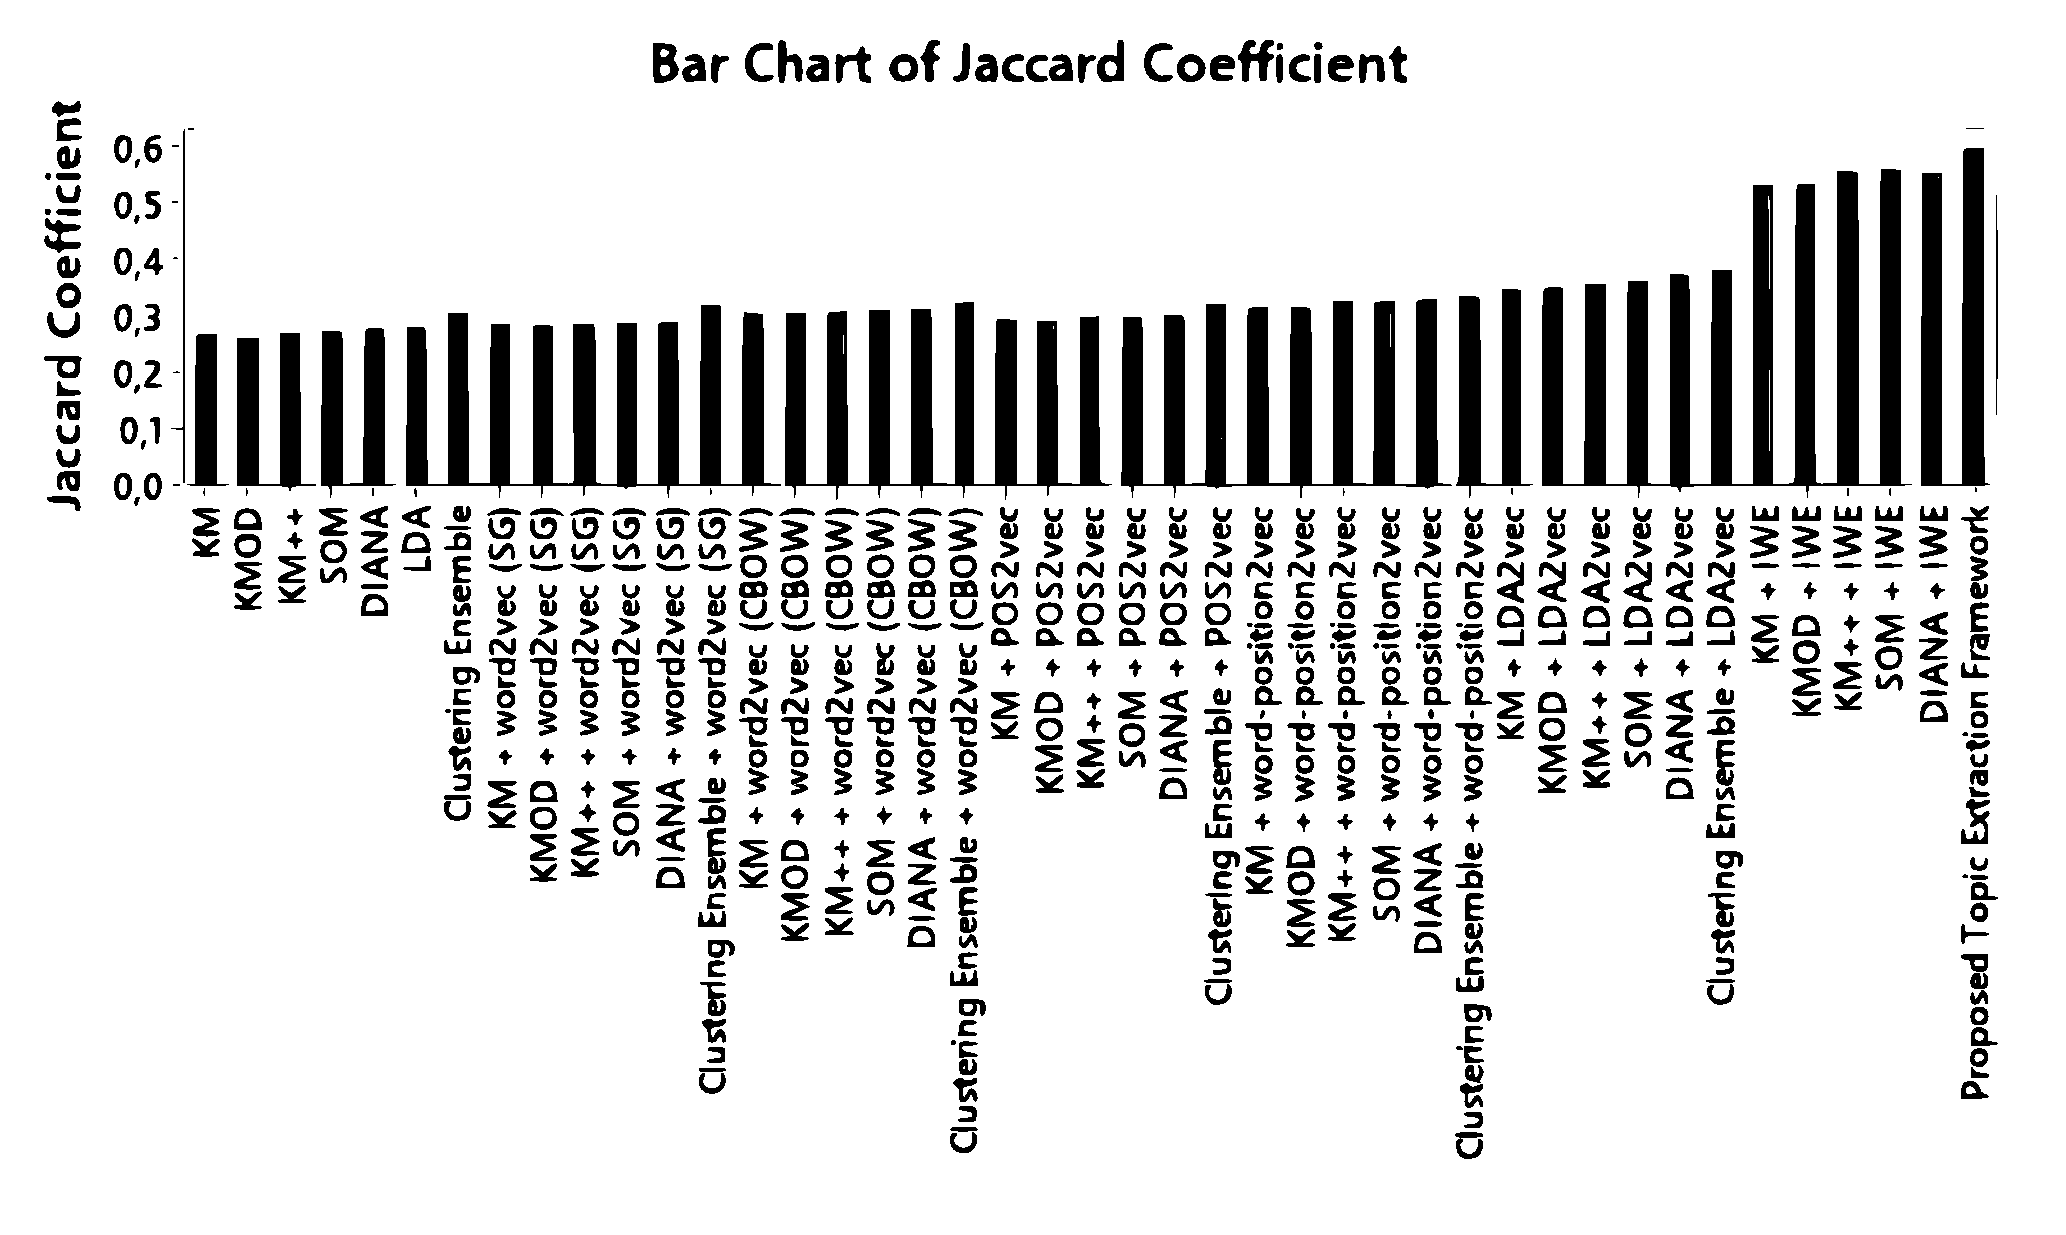
\includegraphics[width=0.75\textwidth]{./visuals/gr1.pdf}}
	\caption{Jaccard Coefficient metric for different combinations of embedding and clustering methods (from \cite{onan2019two}).}
\label{fig:gr1}
\end{figure}

As opposed to the example presented above, topic analysis can solve not only the problem of extracting broad semantic themes from texts but also some more nuanced information. Authors of the article \cite{huang2020weakly} propose their two-step approach for aspect-based sentiment analysis. Their procedure lets evaluate reviews in terms of how positive or negative they are and also define aspects of the review object which are evaluated. In the publication, restaurant and laptop reviews were used as input data. The proposed model outputs a tuple in form of (sentiment, aspect). For example, a review of a restaurant could output (good, ambiance) or (bad, food).

For this finesse task a two-step procedure called JASen was developed. It consists of sentence embedding and classification via convolutional neural networks (CNNs). The former takes labeled data for embedding training and unlabeled data for further classification.

The results shown by the JASen model were compared with those of previously developed approaches. Values of aspect identification and sentiment polarity classification are presented in the tables \ref{tab:t1} and \ref{tab:t2} below (\cite{huang2020weakly}).

\begin{table}[h]
\centering
\caption{Quantitative evaluation on aspect identification, \% (from \cite{huang2020weakly}).}
\label{tab:t1}
\resizebox{0.8\columnwidth}{!}{
\begin{tabular*}{\hsize}{@{\extracolsep{\fill}}lllllllll@{}}
\toprule
\multirow{2}{*}{Methods} & \multicolumn{4}{c}{Restaurants}          & \multicolumn{4}{c}{Laptops}              \\ 
                         & Accuracy & Precision & Recall & F1 & Accuracy & Precision & Recall & F1 \\
\colrule
CosSim & 61.43 & 50.12 & 50.26 & 42.31 & 53.84 & 58.79 & 54.64 & 52.18 \\
W2VLDA & 70.75 & 58.82 & 57.44 & 51.40 & 64.94 & 67.78 & 65.79 & 63.44 \\
BERT & 72.98 & 58.20 & \textbf{74.63} & 55.72 & 67.52 & 68.26 & 67.29 & 65.45 \\
JASen & \textbf{83.83} & \textbf{64.73} & 72.95 & \textbf{66.28} & \textbf{71.01} & \textbf{69.55} & \textbf{71.31} & \textbf{69.69} \\
\botrule
\end{tabular*}
}
\end{table}

\begin{table}[h]
\centering
\caption{Quantitative evaluation on sentiment polarity classification, \% (from \cite{huang2020weakly}).}
\label{tab:t2}
\resizebox{0.8\columnwidth}{!}{
\begin{tabular*}{\hsize}{@{\extracolsep{\fill}}lllllllll@{}}
\toprule
\multirow{2}{*}{Methods} & \multicolumn{4}{c}{Restaurants}          & \multicolumn{4}{c}{Laptops}              \\ 
                         & Accuracy & Precision & Recall & F1 & Accuracy & Precision & Recall & F1 \\
\colrule
CosSim & 70.14 & 74.72 & 61.26 & 59.89 & 68.73 & 69.91 & 68.95 & 68.41 \\
W2VLDA & 74.32 & 75.66 & 70.52 & 67.23 & 71.06 & 71.62 & 71.37 & 71.22 \\
BERT & 77.48 & 77.62 & 73.95 & 73.82 & 69.71 & 70.10 & 70.26 & 70.08 \\
JASen & \textbf{81.96} & \textbf{82.85} & \textbf{78.11} & \textbf{79.44} & \textbf{74.59} & \textbf{74.69} & \textbf{74.65} & \textbf{74.59} \\
\botrule
\end{tabular*}
}
\end{table}

This way, the authors have proposed a model fine-tuned for joint aspect-sentiment extraction which outperformed earlier methods for this task.

However, more often the extraction of topics is enough. In contrast to the ensemble approach proposed in the publication \cite{onan2019two}, authors of the article \cite{grootendorst2022bertopic} leverage different modified algorithms that compose BERTopic -- a modern and efficient topic analysis tool.

Its defining feature is the ability to extract topics dynamically and to build topic popularity time series. This is allowed by using c-TF-IDF (class term frequency inverse document frequency) representations of topics defined by equation \ref{eq:ta4}.
\begin{equation} \label{eq:ta4}
\mathrm{c\_TF\_IDF} = \underbrace{\frac{n_t}{\sum\limits_{k \in \mathrm{class}} n_k}}_{\textrm{c-TF}} \cdot \underbrace{\log \left[ \frac{|D|}{|\{ d_i \in D | t \in d_i \}|} \right]}_{\mathrm{IDF}}
\end{equation}
Here c-TF is defined by the number of instances of word $t$ divided by the number of words in the class, $|D|$ - number of documents in the dataset, $|\{ d_i \in D | t \in d_i \}|$ -- number of documents in dataset, containing the word $t$. First, BERTopic is fitted on the entire dataset to create a global view of topics. Using c-TF-IDF is efficient, as IDF is computed globally and only c-TF needs to be computed at each timestep.

In the publication, newly proposed BERTopic is compared to its predecessors: LDA, NMF, top2vec and CTM by means of topic coherence (TC) and topic diversity (TD) metrics on three datasets of news and twitter posts. According to the article, BERTopic has high coherence scores across all datasets. In terms of topic diversity, it is outperformed by CTM.

One of the major strengths of BERTopic is that it has the capability to operate in the multilingual mode. The default embedding model ``all-MiniLM-L6-v2" shows both moderately high topic coherence and diversity across all supported languages in addition to it being lightweight.

More detailed comparison of BERTopic with other methods of topic analysis is presented in the publication \cite{egger2022topic}. The authors have chosen latent Dirichlet allocation (LDA), non-negative matrix factorization (NMF), top2vec and BERTopic in the task of topic analysis on the dataset of Twitter posts.

LDA is a generative probabilistic model for discrete data, which could be viewed as three-level hierarchical Bayesian clustering algorithm. Each document is represented as a mixture of topics with corresponding probabilities and each topic is a mixture over the collection of topic probabilities.

NMF is a decompositional method which works of TF-IDF transformed data by breaking down the input term-document matrix ($A$) into a pair of lower-ranking matrices:
\begin{itemize}
	\item terms-topics ($W$) matrix containing basis vectors;
	\item topics-documents ($H$) matrix containing weights.
\end{itemize}
In NMF all elements in those matrices are non-negative so as to be interpretable.

Top2vec algorithm uses word embeddings via pretrained embedding models so that semantically close words have spatially close embedding vectors. Due to the sparsity of the vector space, a dimension reduction is performed before clustering. Commonly, hierarchical density-based spatial clustering of applications with noise (HDBSCAN) is used to identify dense regions in the reduced vector space of documents. As words that appear in several documents cannot be assigned to one document, they are recognized as noise. Thus, no lemmatization is needed beforehand.

BERTopic uses BERT (bidirectional encoder representations from transformers) pretrained embedders alongside with sentence-transformers for turning documents into vectors across more than 50 languages. Similarly to top2vec, BERTopic uses uniform manifold approximation and projection (UMAP) for dimension reduction and HDBSCAN for clustering. The principal difference between BERTopic and top2vec is that the latter utilizes c-TF-IDF metric instead of normal TF-IDF. Thus, importance of words in clusters and not in documents is taken into account. The usage of HDBSCAN eliminates the need for lemmatization.

Human interpretation of the extracted topics has shown that BERTopic and NMF perform the best among four tested methods. Despite that top2vec and BERTopic both use pretrained embedders for the representation of documents in vector space, many topics extracted by top2vec contained several semantic concepts or intersected each other. LDA gave the least legible results of all methods.

The authors mentioned several drawbacks of BERTopic models such as them yielding large numbers of clusters which leads to the need in manual topic processing. Another mentioned disadvantage is that one document could potentially be assigned to just one topic, which often does not reflect reality. In spite of this, BERTopic still can be characterized as one of the most successful and universally applicable methods of topic analysis due to high model quality and efficiency.

\subsubsection{Time series prediction} \label{tsp}

Time series forecasting is one of the most important tasks related to time-dependent processes. A plethora of methods for predicting time series have been developed and the most practical ones were described in the publication \cite{parmezan2019evaluation}. The authors group all methods into two major categories: parametric and non-parametric.

Among the parametric methods the following were described:
\begin{enumerate}
\item \underline{Moving averages} models (MA), simple models that view predicted values at a certain timestep as averages over some interval before this step. MA model is defined by the equation \ref{eq:tsp1}.
\begin{equation} \label{eq:tsp1}
z_{t+1} = \frac{\sum\limits_{i=0}^{r-1}z_{t-i}}{r}
\end{equation}
Here, $t$ is the timestep, $z_{t+1}$ is the predicted value and $r$ is the number of observations included in the average. Such models are simple but lack quality, when data has seasonality, trend or high-frequency noise.
\item \underline{Simple exponential smoothing} models (SES) are conceptually close to MA. The main difference is that all previous timesteps are taken into account with different weights, which exponentially decrease the further away from prediction the timestep is. They are defined by the equation \ref{eq:tsp2}.
\begin{equation} \label{eq:tsp2}
z_{t+1} = L_t = \sum_{i=0}^{t-1} \alpha (1-\alpha)^i z_{t-i}
\end{equation}
Here $\alpha \in (0,1)$ is the weight for constant smoothing and $L_t$ is the estimate for the next step at time $t$. For ease of computation, recurrent simplification can be formalized by equation \ref{eq:tsp3}.
\begin{equation} \label{eq:tsp3}
L_t = \alpha z_t + (1-\alpha) L_{t-1}
\end{equation}
Initially, it is supposed that $L_1 = z_1$. The main drawback of the method is the difficulty in optimizing $\alpha$ and inaccurate results when dealing with trends.
\item \underline{Holt's exponential smoothing} (HES) is an extension of SES that utilizes a second smoothing constant $\beta$ for modeling trends. HES models are defined by equations \ref{eq:tsp4} -- \ref{eq:tsp6}.
\begin{equation} \label{eq:tsp4}
L_t = \alpha z_t + (1-\alpha) (L_{t-1} + T_{t-1})
\end{equation}
\begin{equation} \label{eq:tsp5}
T_t = \beta (L_t - L_{t-1}) + (1-\beta) T_{t-1}
\end{equation}
\begin{equation} \label{eq:tsp6}
z_{t+h} = L_t + hT_t
\end{equation}
Here, $L$ and $T$ are the level and trend components, accordingly, and $h$ is the prediction horizon (more than 1 step as opposed to SES). Initially, $L_1 = z_1$ and $T_1 = z_2 - z_1$. As in SES method, the most difficult part is the optimization of $\alpha$ and $\beta$ constants.
\item \underline{Holt-Winters' seasonal exponential smoothing} models (HW) iterate on HES method principles and additionally deal with seasonality by adding another constant $\gamma$. More commonly used additive HW models (AHW) are defined by equations \ref{eq:tsp7} -- \ref{eq:tsp10}.
\begin{equation} \label{eq:tsp7}
L_t = \alpha (z_t - S_{t-s}) + (1-\alpha) (L_{t-1} + T_{t-1})
\end{equation}
\begin{equation} \label{eq:tsp8}
T_t = \beta (L_t - L_{t-1}) + (1-\beta) T_{t-1}
\end{equation}
\begin{equation} \label{eq:tsp9}
S_t = \gamma (z_t - L_t) + (1-\gamma) S_{t-s}
\end{equation}
\begin{equation} \label{eq:tsp10}
z_{t+h} = L_t + hT_t + S_{t-s+h}
\end{equation}
Here, $S$ is the seasonal component and $s$ denotes the number of timesteps that make a full seasonal cycle. $L$ is usually initialized by the equation \ref{eq:tsp11}.
\begin{equation} \label{eq:tsp11}
L_s = \frac{1}{s} \sum_{i=1}^s z_i
\end{equation}
$T$ with equation \ref{eq:tsp12}.
\begin{equation} \label{eq:tsp12}
T_s = \frac{1}{s} \sum_{i=1}^s \frac{z_{s+i} - z_i}{s}
\end{equation}
and $S$ indexes are computed according to equation \ref{eq:tsp13}:
\begin{equation} \label{eq:tsp13}
S_i = z_i - L_s, \quad i \in [1,s]
\end{equation}
\item (S)ARIMA, \underline{(seasonal) autoregressive integrated moving average} models provide even higher quality forecasts for stochastic time series and conceptually include three operations: autoregression AR with parameter $p$, intergration I with parameter $d$ and moving averages MA with parameter $q$. Here, integration refers to taking successive differences from the time series ($\Delta z_t = z_t - z_{t-1}$) so as to make the time series stationary, i.e. with no trend and constant deviation. ARIMA of order $(p,d,q)$ is defined by the equation \ref{eq:tsp14}.
\begin{equation} \label{eq:tsp14}
I'_t = \Delta^d z_t = \delta + \sum_{i=1}^p \varphi_i I'_{t-i} + \sum_{i=1}^q \theta_i e_{t-i} + e_t
\end{equation}
Here, $I'_t$ is the value of the $d$-times differenced stationary time series, $\varphi_i$ are AR parameters with lags up to $p$ and $\theta_i$ are MA parameters with lags up to $q$. Parameter $\delta$ is the initial level of the model and the last term $e_t$ denotes white noise with zero mean and constant deviation. If $d>1$, the constant $\delta$ can be omitted.
SARIMA model is an extension of ARIMA that takes in four additional parameters and models seasonality. It is essentially ARIMA $(p,d,q)$ with a seasonal part added. SARIMA of order $(p,d,q)\times (P,D,Q)_s$, where $P$, $D$ and $Q$ are maximum lags of AR, differencing degree and maximum lags of MA of the seasonal component denoted as $I''_t$ below \ref{eq:tsp15}.
\begin{equation} \label{eq:tsp15}
I_t = \underbrace{\delta + \sum_{i=1}^p \varphi_i I'_{t-i} + \sum_{i=1}^q \theta_i e_{t-i} + e_t}_{\mathrm{ARIMA}} + \underbrace{\sum_{i=1}^P \Phi_i I''_{t-is} + \sum_{i=1}^Q \Theta_i e_{t-is}}_{I''_t = \Delta^D z_t}
\end{equation}
As in ARIMA, here $\delta$ can be omitted if $d+D > 1$. (S)ARIMA models are the most commonly used methods of time series forecasting in the modern practice due to algorithm efficiency, ease of use and high quality of predictions on a large range of time series.
A detailed usage example of ARIMA on the COVID-19 epidemic dataset is presented in the publication \cite{benvenuto2020application}. In the article, as ARIMA is a widely-used model utilized for time series forecasting, no testing of the model was presented. The authors predicted values for the differenced COVID-19 dataset and provided confidence intervals for the forecast. This, as well as the autocorrelation analysis before model fitting gives insight into the real-world usage of ARIMA models on actual data, which provides estimations for the future. 
\end{enumerate}

In addition, the authors gave a brief description of non-parametric methods for forecasting processes, which include the following:
\begin{enumerate}
	\item \underline{Artificial neural networks} (ANNs) are models comprised of neurons -- objects capable of taking several inputs, combining them linearly with a certain bias and feeding the output to an activation function (often sigmoid or relu). The output of a single neuron can be described by the equation \ref{eq:tsp16}.
\begin{equation} \label{eq:tsp16}
f(\mathrm{net}) = f\left( \sum_{i=1}^l w_i x_i + b \right)
\end{equation}
Here, $x_i$ and $w_i$ are inputs and weights, $b$ is a bias and $f$ is the activation function. Arranging neurons in several layers (multiple layer perceptron, MLP) was allowed by introducing backpropagation learning algorithms, where the weights are adjusted to better fit the data in reverse layer order.
An example usage of multilayer feed-forward neural networks (MLFFNN) is presented in the publication \cite{khosravi2018time}. The authors showed that even such simple architecture of ANNs can produce good quality forecasts. The paper contains R-metrics (correlation coefficients between predictions and test data) for a dataset of wind speed time series for MLFFNN with values as high as 0.9995.
In addition, the authors suggest adaptive neuro-fuzzy inference system (ANFIS) -- a method that combines ANNs with fuzzy inference system. The latter implies the usage of fuzzy-parameters (if-else rules manually trained by specialists in the research field). According to the results presented in the article, the utilization of such rules slightly improves time series prediction as opposed to MLFFNN.
In the networks mentioned above, neuron-to-neuron signals flow only from input to output. This does not apply to recursive neural networks (RNNs), where neurons form a cycle and the signal has several flow directions. In the simple recurrent network (SRN), the state of a chosen layer within a cycle is conditioned by a context layer on its previous state. This creates short-term memory, i.e. the ability of the network to store complex signals.
The most advanced RNNs for forecasting time series are the long short-term memory (LSTM) networks. LSTMs are described by the authors of the publication \cite{hua2019deep} as essentially RNNs tuned for learning long-term dependencies via components called ``memory blocks". The latter are recurrent subnets comprised of memory cells and gates. Memory cells' role is to remember the current state of the network and the gates are in charge of controlling the flow of signal in the network. By their role, gates are classified as input (control the amount of new input data that flows into the network), output (the amount of information that flows out of the memory block) and forget gates (decide the amount of information that remains in the current cell). The layout of a memory block is presented in figure \ref{fig:gr2} (\cite{hua2019deep}).
\begin{figure}[t]\vspace*{4pt}
%\centerline{\includegraphics{fx1}\hspace*{5mm}\includegraphics{fx1}}
	\centerline{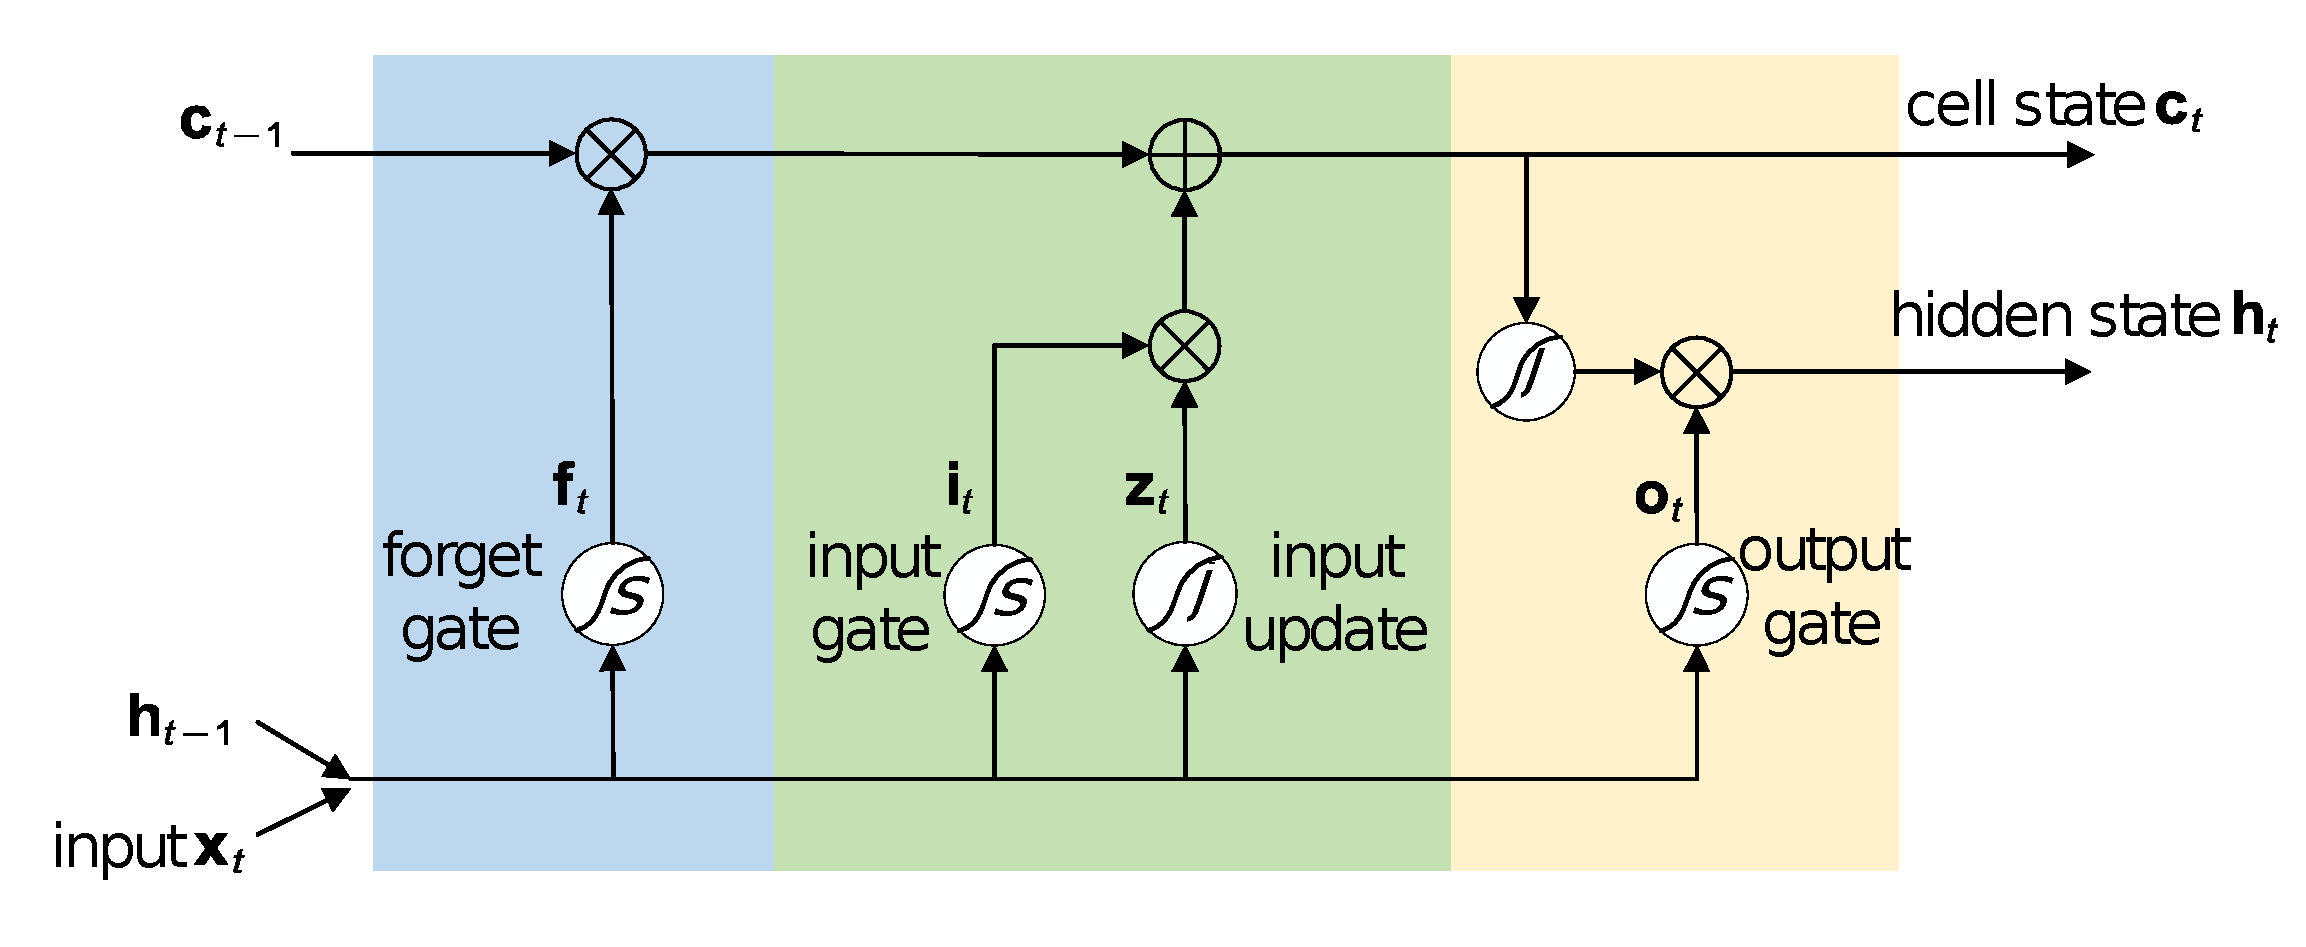
\includegraphics[width=0.75\textwidth]{./visuals/gr2.pdf}}
	\caption{An illustration of LSTM memory block (from \cite{hua2019deep}).}
\label{fig:gr2}
\end{figure}
It is first decided, which old information stays in the cell, then new information is chosen to be stored. Updating of the cell state is performed by multiplying the old memory state by the forget gate output. Then the element-wise product of the input gate and the candidate values for the new information is added. This procedure lets LSTMs predict time-series with long-term dependencies. Several architectures of LSTM models exist that differ by how the neurons in each memory block are connected. As opposed to fully-connected neurons in the traditional LSTM, they are randomly connected in randomly connected LSTMs (RCLSTM), proposed by the authors of the paper \cite{hua2019deep}. This architecture more closely resembles real synapses in the human brain, which was one of the reasons for the proposal. The authors tested RCLSTM on several datasets including a dataset of traffic information. The influence of the percentage of connected neurons on the predictive quality was estimated my comparison of RMSE metrics. RCLSTM took less computational resources than standard LSTM, however seemed to be outperformed by it. Taking the above into account, RCLSTM still showed better predictions than commonly used methods such as SVR (support vector machines), ARIMA and FFNN (feed-forward neural networks). This implies that random connection of neurons within LSTMs lets significantly reduce computing time while slightly compromising quality.
Even more structurally complicated versions of LSTMs exist. The authors of \cite{liang2018geoman} suggested GeoMAN ("multi-level attention network to predict the the readings of a geo-sensor..."), that is tuned for spatio-temporal correlations. In the paper the authors test this network on a set of geosensors, each providing time-dependent signals (time series). The network utilizes the multi-level attention mechanism including local and global spatial attention as well as temporal attention. This lets the network extract both correlations between different geosensors and also within one time series. Additionally, the authors implemented external factor fusion module, a mechanism of including exogenous variables from different domains for better predictions. The actual architecture of the GeoMAN model is depicted in the figure \ref{fig:gr3} (\cite{liang2018geoman}).
\begin{figure}[h!]\vspace*{4pt}
%\centerline{\includegraphics{fx1}\hspace*{5mm}\includegraphics{fx1}}
	\centerline{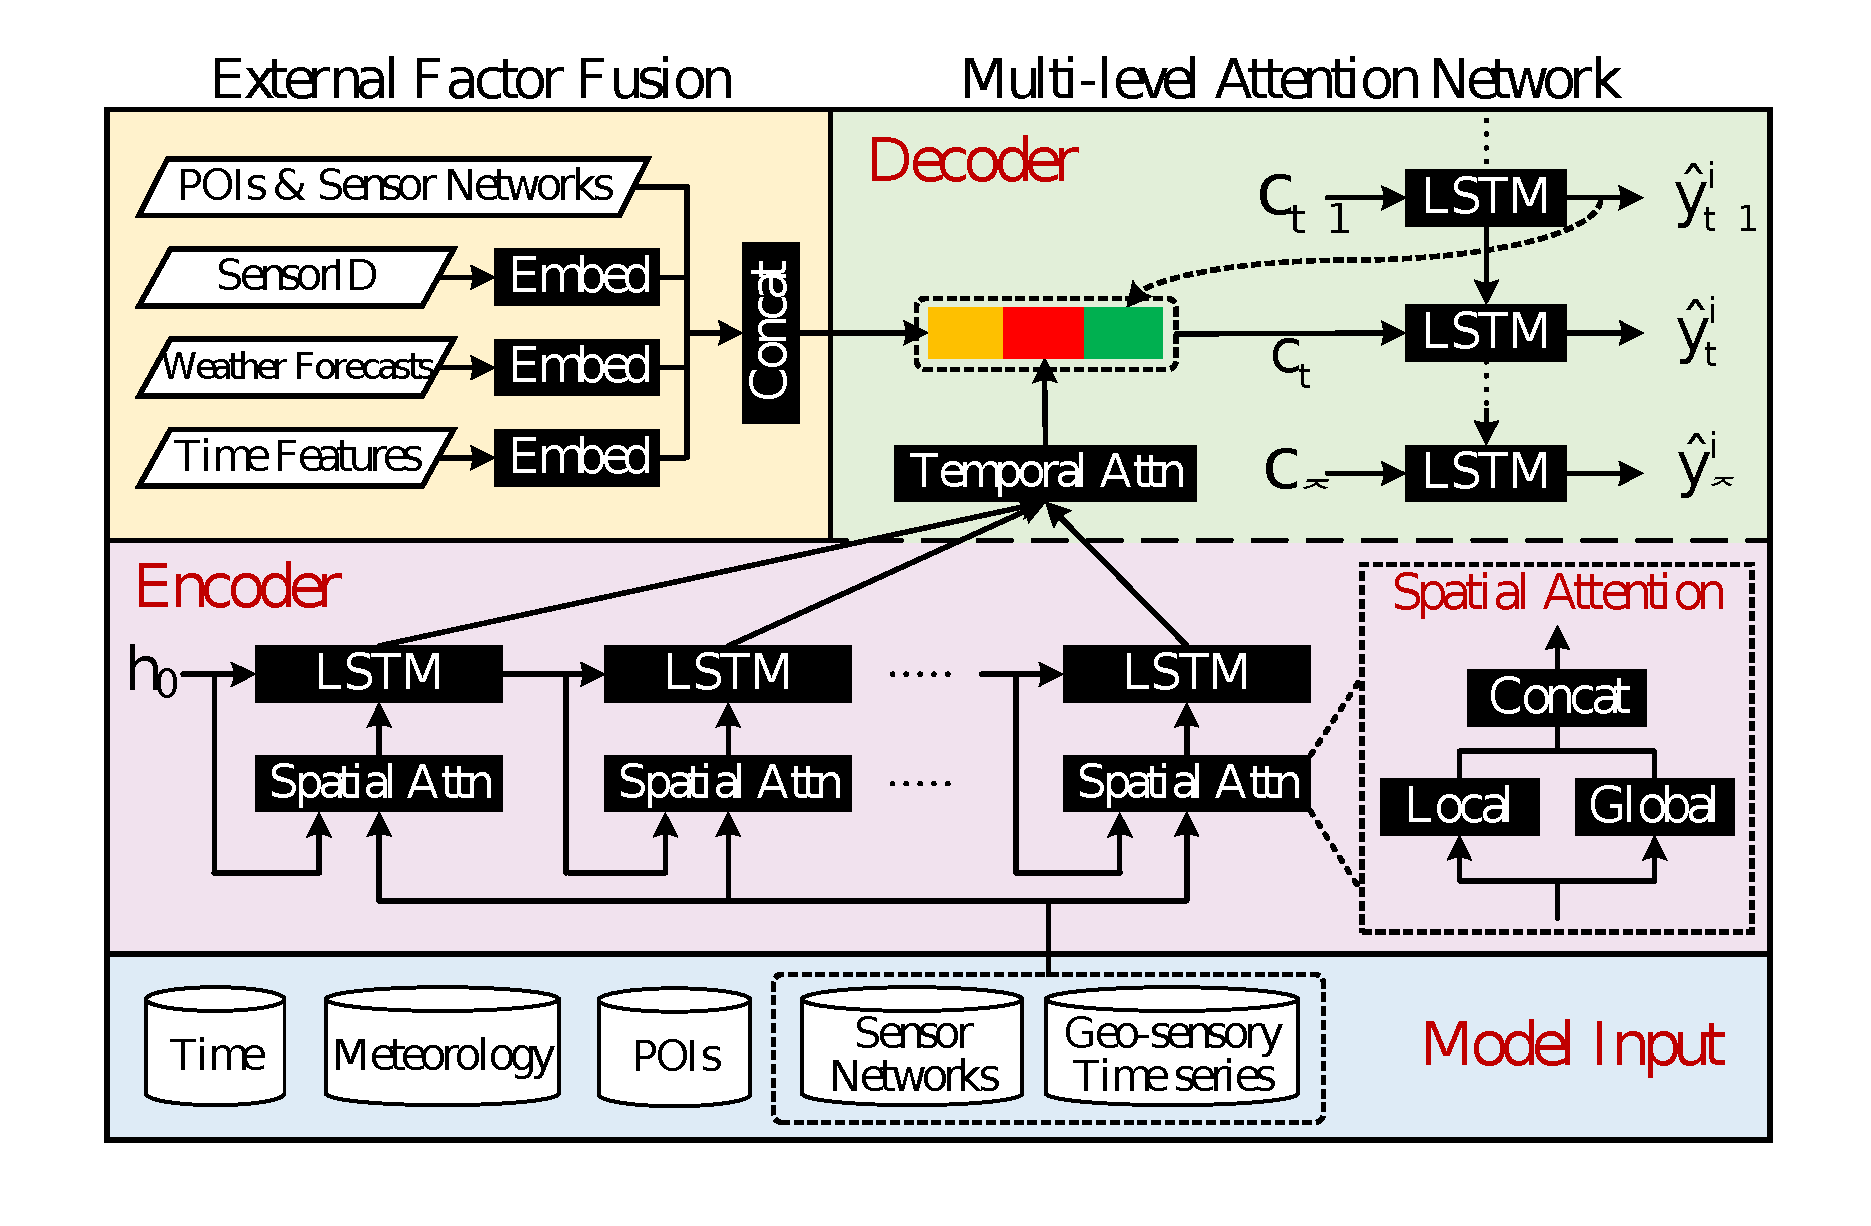
\includegraphics[width=0.7\textwidth]{./visuals/gr3.pdf}}
	\caption{The framework of GeoMAN (from \cite{liang2018geoman}).}
\label{fig:gr3}
\end{figure}

It can be essentially broken down to two LSTM models, one acting as an encoder for spatial attention and the other as a decoder for temporal. The model was tested on spatio-temporal datasets of water and air quality and within the experiment it was also compared to nine commonly used baseline models including ARIMA, VAR (vector auto-regressive) and many variations of RNNs. According to the publication, on spatio-temporal data GeoMAN outperforms all baseline models, both parametric and non-parametric, judging by RMSE values. Thus, the paper \cite{liang2018geoman} proves that RNN models can be effectively engineered to perform well on spatio-temporal data.
\item \underline{Support vector machines} (SVMs) are algorithms conceptually close to ANNs but minimizing the training error while also minimizing the upper bound on the error when the model is applied to test data. The classical illustration to SVMs, binary classification, is presented in figure \ref{fig:gr4} (\cite{parmezan2019evaluation}).
\begin{figure}[h!]\vspace*{4pt}
%\centerline{\includegraphics{fx1}\hspace*{5mm}\includegraphics{fx1}}
	\centerline{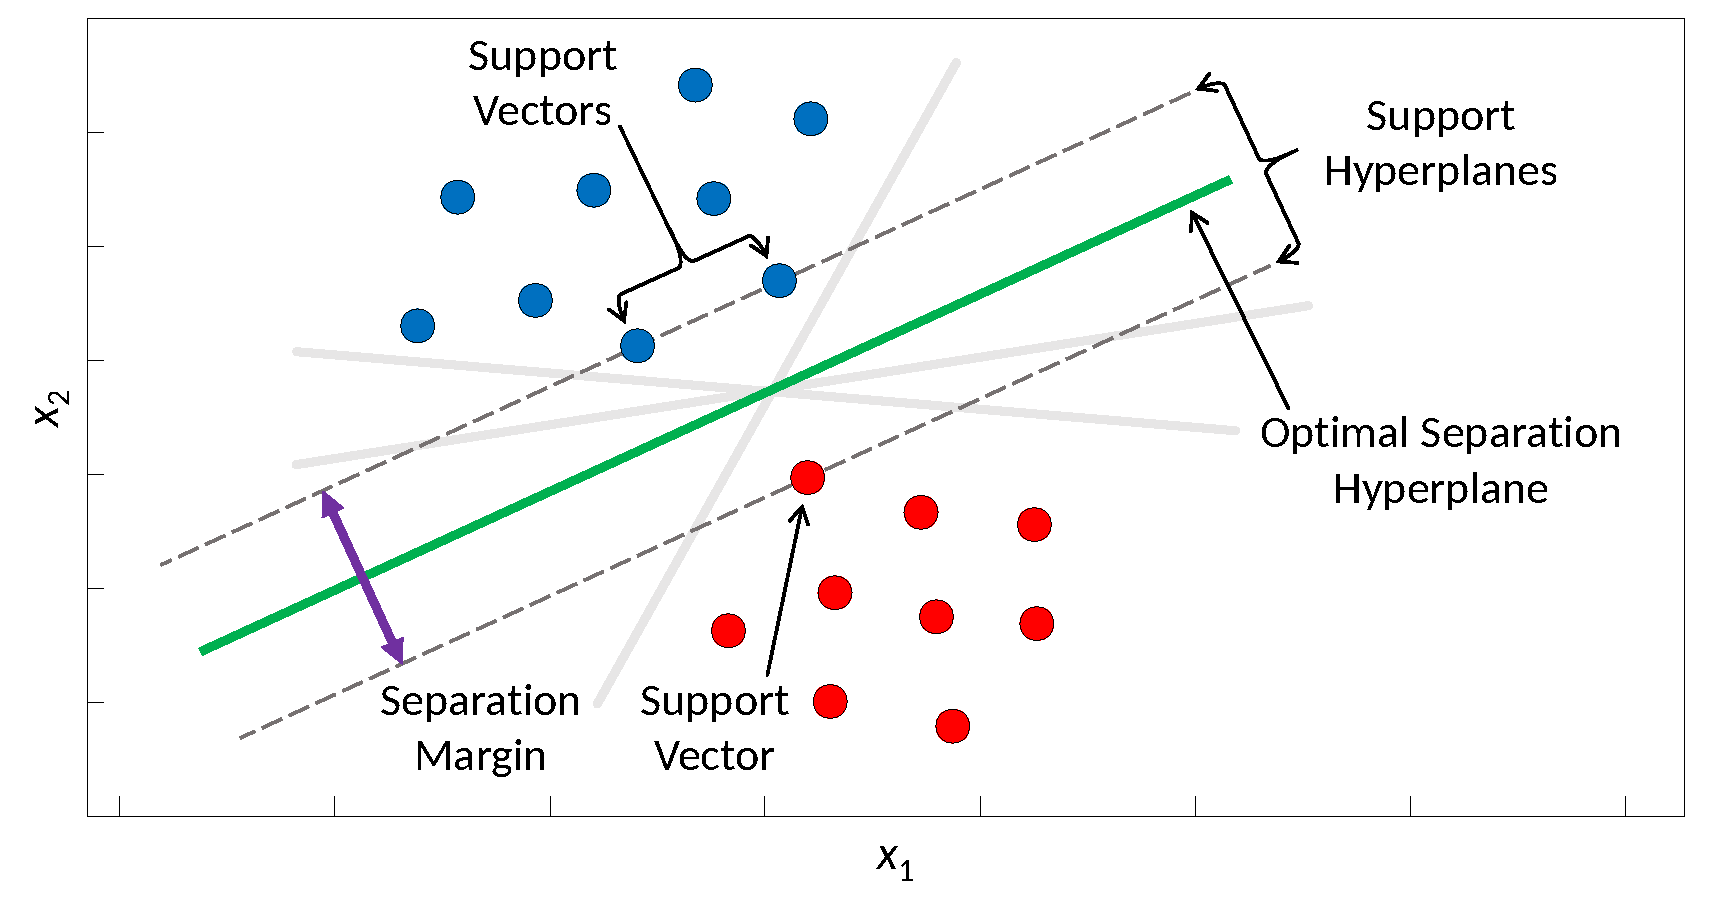
\includegraphics[width=0.65\textwidth]{./visuals/gr4.pdf}}
	\caption{Binary classification using support vector machines (from \cite{parmezan2019evaluation}).}
\label{fig:gr4}
\end{figure}

The figure shows a set of hyperplanes dividing the two classes. An SVM seeks the optimal divider, where the highest separation margin (distance from divider to support vectors) is reached.
As a part of a broader research, SVMs are used along other models in the publication \cite{khosravi2018time} for predicting wind speeds. It showed highly accurate predictions with $R$-statistics of up to $0.9938$, which is accurate, albeit less accurate than the other methods that comprised the research in \cite{khosravi2018time}. 
\item \underline{$k$-nearest neighbors} ($k$NN) are in nature similarity-based classification algorithms. For forecasting $z_{m+1}$ for a time series $Z = (z_1, \cdots, z_m)$ the algorithm uses last $l$ timesteps as query $Q$ and searches for $k$ most similar subsequences to $Q$ by sliding a window of size $l$ along the time series. Then, the values of $S_{l+1}^{(j)}$ are averaged in an ensemble to predict $z_{m+1}$ as depicted in equation \ref{eq:tsp17}.
\begin{equation} \label{eq:tsp17}
f(S) = \frac{1}{k} \sum_{j=1}^k S_{l+1}^{(j)}
\end{equation}
Such $k$NN models have shown the capability to model highly complex non-linear patterns, especially in form of time series prediction with invariance $k$NN ($k$NN-TSPI). The later algorithm deals with trivial matches, amplitude, offset and complexity invariance.
\item The authors of the publication \cite{rangapuram2018deep} offered a hybrid method that combined \underline{state space models} (SSMs) with deep neural networks. Principally, SSMs utilize a latent space that is used to encode time series' features: level, trend and seasonality. Linear SSMs are described by the equation \ref{eq:tsp18}.
\begin{equation} \label{eq:tsp18}
\mathbf{l}_t = \mathbf{F}_t\mathbf{l}_{t-1} + \mathbf{g}_t \varepsilon_t, \quad \varepsilon_t \sim \mathcal{N} (0,1)
\end{equation}
Here, $\mathbf{l}_t$ is the state of the latent space at timestep $t$, $\mathbf{F}_t$ is a deterministic transition matrix and $\mathbf{g}_t \varepsilon_t$ is a random innovation. The predicted value is defined by the equation \ref{eq:tsp19}.
\begin{equation} \label{eq:tsp19}
z_t = \mathbf{a}_t^\top \mathbf{l}_{t-1} + b_t + \sigma_t \varepsilon_t, \quad \varepsilon_t \sim \mathcal{N} (0,1)
\end{equation}
Here, $\mathbf{a}^\top \in \mathbb{R}^L$, $\sigma_t \in\mathbb{R}^{>0}$ and $b_t \in \mathbb{R}$ are time-varying parameters of the model.
SSMs in general are optimized for applications where the time series are structured and this structure is well-known. The major drawback of SSMs is that multivariate analysis of several correlated time series is impossible as the model if fitted onto one process at a time. In the publication, a hybrid model is proposed, that takes advantage of the benefits of both SSMs and RNNs. The model is comprised of an RNN that is used to parametrize a particular linear SSM. RNN's parameters are learned simultaneously from the whole dataset with all additional covariates, which lets the extraction of shared patterns.

This ``orchestration" of several SSMs with an RNN is a complicated model architecture, which was quantitatively tested by the authors of the paper \cite{rangapuram2018deep} against more conventional baseline models such as ARIMA and DeepAR, an RNN-based method. The models were used to forecast electricity consumption and traffic occupancy rates. They were compared by the values of standard $p50$ and $p90$ quantile loss metrics. On the one hand, the majority of the tests with forecasting long-term horizons showed that the proposed hybrid method slightly outperformed the others. On the other hand, DeepAR -- RNN -- performed better at predicting a short forecast horizon.
\end{enumerate}

The methods of time series forecasting as well as some of their traits were gathered in the table \ref{tab:t3} for quick reference.

\begin{table}[h]
\centering
\caption{Comparison of time series forecasting methods.}
\label{tab:t3}
\resizebox{0.8\columnwidth}{!}{
	\begin{tabular*}{\hsize}{@{\extracolsep{\fill}}l p{1.5cm} p{5cm} p{5cm} p{2cm} @{}}
\toprule
Method & Type & Benefits & Drawbacks & References \\
\colrule
MA & param. & simple implementation & no trend, seasonality and noise support & \cite{parmezan2019evaluation} \\
SES & param. & simple recurrent implementation & difficulties with trends & \cite{parmezan2019evaluation} \\
HES & param. & simple recurrent implementation & difficulties with seasonality & \cite{parmezan2019evaluation} \\
HW & param. & efficient recurrent implementation & no way to deal with non-stationary data & \cite{parmezan2019evaluation} \\
(S)ARIMA & param. & accurate for stationary time series, can model seasonality, efficient & can be outperformed by artificial neural networks in some cases & \cite{parmezan2019evaluation} \\
\colrule
ANNs & non-param. & high performance of RNNs and even some feed-forward networks such as MLFFNN, complex non-linear pattern modeling of LSTM and similar short-term memory models & take time for optimization, especially architecturally complicated models & \cite{parmezan2019evaluation}, \cite{hua2019deep}, \cite{liang2018geoman} \\
SVMs & non-param. & high accuracy & limited scope of usage (tasks have to be narrowed down to regression or classification) & \cite{parmezan2019evaluation}, \cite{khosravi2018time} \\
$k$NN & non-param. & simple implementation, effectiveness, ability to model non-linear patterns & predictions can be disrupted by anomalies in the data & \cite{parmezan2019evaluation} \\
SSMs & non-param. & good performance on short forecasting horizons & gets outperformed by conventional methods on medium and long horizons & \cite{rangapuram2018deep} \\
\botrule
\end{tabular*}
}
\end{table}

\subsubsection{Prediction with exogenous variables} \label{pwev}

According to \cite{smelser2001international}, ``the variables that show differences we wish to explain are called endogenous, while the variables used to explain the differences are  called exogenous". If a hypothesis exists, that the observed changes in any variable (called endogenous) are caused by changes in some other variables, the latter are referred to as exogenous.

Victor Gijsbers, the author of the publication \cite{gijsbers2021perceiving}, elaborates on the concept of causality and it being perceived. According to the paper and despite the arguments againt the Humean regularity theory that views any perception of a cause-effect pair as universal, experiencing causation leaves open the possibility that either the causality itself or its experience depend on some external events. This implies, that at least for statistical data on human behavior, which cannot be considered strongly local, the perception of causality ($a^* \to b^*$) can theoretically be generalized to ($A \to B$). Here, $a^*$ and $b^*$ denote specific local observations of random variables $A$ and $B$, while the arrow depicts causality.

Thus, if the chosen exogenous variables either cause the changes in the predicted variables or have an indirect impact on them, the usage of such variables in a forecasting model can increase its performance. An example of such increase is presented in the publication \cite{verma2022arima}. The authors tested ARIMA and ARIMAX, the latter being the same autoregressive model but capable of including exogenous context, in the task of sugarcane yield forecasting in Haryana, India. According to the article, ARIMAX, utilizing exogenous weather data for fitting the model, showed consistently better results than the baseline ARIMA. The values of RMSE, used to compare the models, are given in table \ref{tab:t4} (\cite{verma2022arima}).

\begin{table}[!h]
\centering
\caption{Comparative view in terms of RMSEs of sugarcane yield forecasts based on ARIMA and ARIMAX models (from \cite{verma2022arima}).}
\label{tab:t4}
\resizebox{0.8\columnwidth}{!}{
\begin{tabular*}{\hsize}{@{\extracolsep{\fill}}lll@{}}
\toprule
\multirow{2}{*}{District} & \multicolumn{2}{c}{RMSE} \\
 & ARIMA & ARIMAX \\
\colrule
Karnal & 7.44 & 4.18 \\
Ambala & 6.07 & 4.30 \\
Kurukshetra & 9.32 & 6.62 \\
\botrule
\end{tabular*}
}
\end{table}

ARIMAX is one of the most widely used models for forecasting with exogenous context, however, many of the methods described in subsection \ref{tsp} allow for the usage of such variables. The authors of the article \cite{da2020forecasting}, however did not compare models with exogenous variables to those without them, utilized context information for all of their forecasts across five methods in two variations. This includes:
\begin{enumerate}
	\item BRNN -- bidirectional recurrent neural networks are RNNs that allow both positive and negative time directions. This lets future information (such as future values of exogenous variables) to be included at a certain time frame.
	\item CUBIST is rule-based forecasting algorithm that establishes regression models with certain rules based on the input data. General linear regression was used in the paper \cite{da2020forecasting}. Despite the non-linear nature of some time series, implementation of the rules mentioned above lets CUBIST fit complicated temporal patterns.
	\item $k$NN -- $k$-nearest neighbors method described in subsection \ref{tsp} allows for exogenous variables without major modifications as the latter can be used in the $Q$-queries alongside predicted variables.
	\item QRF -- quantile random forest is an extension of the random forest (RF) ensemble learning model. In the QRF algorithm, conditional quantiles are utilized. In contrast to conventional RF models, QRF uses full conditional distribution of the predicted variables instead of just the mean.
	\item SVR -- support vector regression also described in subsection \ref{tsp} similarly to $k$NN is capable of taking in exogenous variables as-is.
\end{enumerate}
All of the models were used both with and without data preprocessing via variational mode decomposition (VMD). It decomposes a time series into a certain number of mode functions with different sparsities.

The authors of the paper \cite{da2020forecasting} tested the mentioned models against each other in the task of predicting COVID-19 cases in Brazil and USA. Climatic data was used as exogenous variables. According to the results presented in the article, the best predictions for each state in both countries had low values of RRMSE (no more than 6.29\% but generally between 1 and 3\%). This implies high predictive qualities of models fit with help of exogenous variables, even on large forecast horizons.

Many more variations of autoregressive models that have the capability of including exogenous variables exist. For example, the author of the Master's thesis \cite{ding2021empirical} utilized VARX (vector autoregression with exogenous variables) for predicting stocks and CDS. VARX is an extesion of VAR (vector autoregression) which is closely related to ARIMA. The major benefit of VAR over ARIMA is the capability of multivariate analysis with cross-correlations between different variables. Below, an example equation (\ref{eq:pwev1}) for VARX with two variables is presented.
\begin{equation} \label{eq:pwev1}
\begin{pmatrix}\Delta x_t \\ \Delta y_t \end{pmatrix}
= \begin{pmatrix}\alpha_0 \\ \beta_0 \end{pmatrix}
+ \begin{pmatrix}\sum_{i=1}^p \alpha_{1,i} & \sum_{i=1}^p \alpha_{2,i} \\ \sum_{i=1}^p \beta_{1,i} & \sum_{i=1}^p \beta_{2,i} \end{pmatrix}
\begin{pmatrix}\Delta x_{t-1} \\ \Delta y_{t-1} \end{pmatrix}
+ \begin{pmatrix}\alpha_3 & \alpha_4 \\ \beta_3 & \beta_4 \end{pmatrix}
\begin{pmatrix}\Delta z_{1, t-1} \\ \Delta z_{2, t-1} \end{pmatrix}
+ \begin{pmatrix}\epsilon_t \\ \varepsilon_t \end{pmatrix}
\end{equation}
Here, $x$ and $y$ are endogenous variables, $z_1$ and $z_2$ -- exogenous. Coefficients $\alpha_1$ and $\beta_2$ refer to autoregressive coefficients of $x$ and $y$, accordingly, while $\alpha_2$ and $\beta_1$ are cross-coefficients. The last term in the equation is white noise of the corresponding dimension.

The author used VARX model in the task of predicting CDS and stock prices on the Norwegian market using bond yield and NOK/EUR currency exchange rate (their once-differenced time series) as exogenous variables. According to the thesis, a causal bond between the endogenous variables was found in the way that using exogenous context alongside stock prices as predictors lets accurately forecast CDS, however the opposite is not true. Thus, VARX is a valid method for predicting time series when cross-correlatioins between endogenous variables coexists with important exogenous context. 

Another example of an autoregressive model utilizing exogenous variables is brought up in the publication \cite{li2022nonlinear}. The authors used nonlinear autoregressive (NARX) model which is a modification of simple AR that allowes for:
\begin{enumerate}
	\item exogenous variables;
	\item nonlinearity in time series patterns.
\end{enumerate}
The model is defined by the equation \ref{eq:pwev2}.
\begin{equation} \label{eq:pwev2}
y_t = f(y_{t-i}, x_{k, t-j}), \qquad \begin{matrix}i \in [1, m] \\ j \in [1, n] \\ k \in [1, n] \end{matrix}
\end{equation}
Here, $y$ is endogenous, $x_k$ is exogenous and $f(\cdots)$ is a nonlinear function. The authors of the paper used a focused time-delay neural network (FTDNN) for $f$. The network itself has a complex series-parallel architecture, where the structure of the network changes as the training goes on. According to the article, FTDNN has several advantages over conventionally used RNN including extended capabilities of dealing with short sequence lengths and feature sizes.

The authors tested this NARX model for forecasting traffic flow in the selected portion of a street in the city of Guilin. The model performed reasonably well with $R$ metrics around $0.96$ and showed even better predictions after one differencing of the time series. In comparison to more conventional methods, NARX without differencing showed performance better than Holt-Winters method but worse than SARIMA. NARX with one differencing, however, outperformed both models with the $R^2$ metric reaching the value of $0.957$.

The methods of predicting time series with exogenous context and their traits were summarized in the table \ref{tab:t5} below.

\begin{table}[!h]
\centering
\caption{Comparison of time series forecasting methods \\ that allow for exogenous context.}
\label{tab:t5}
\resizebox{0.8\columnwidth}{!}{
\begin{tabular*}{\hsize}{@{\extracolsep{\fill}}l p{2.5cm} p{4.5cm} p{4.5cm} l@{}}
\toprule
Method & Type & Benefits & Drawbacks & References \\
\colrule
ARIMAX & autoregressive, parametric & effectiveness, higher accuracy than ARIMA & is outperformed by many modern NNs & \cite{verma2022arima} \\
VARX & autoregressive, parametric & exceptional performace, if endogenous variables are cross-correlated & limited scope of usage & \cite{ding2021empirical} \\
NARX & autoregressive, parametric & models non-linear patterns, easy implementation & may not work well with non-stationary data & \cite{li2022nonlinear} \\
\colrule
BRNN & RNN, \newline non-parametric & good performance, inclusion of future information into modeling current timestep & as all RNNs, requires time for fitting & \cite{da2020forecasting} \\
$k$NN & similarity-based, \newline non-parametric & simple implementation & performance depends on anomalies in the training data & \cite{da2020forecasting} \\
QRF & RF, \newline non-parametric & good performance, usage of full conditional distribution of the predicted variables & is outperformed by some ANNs & \cite{da2020forecasting} \\
SVR & SVM, \newline non-parametric & good performance & limited scope of usage (tasks have to be narrowed down to regression or classification) & \cite{da2020forecasting} \\
CUBIST & rule-based & can model complicated patterns & performance depends on rule definition & \cite{da2020forecasting} \\
\botrule
\end{tabular*}
}
\end{table}

\subsubsection{Impact of context information on consumption} \label{icic}

This final part of the literature overview is aimed to combine all the methods mentioned in previous subsections for answering the question, whether it is possible to use news as predictors for forecasting economical time series. This raises several questions, each narrower in nature:
\begin{enumerate}
	\item Do news have enough impact on the consumers to change their behavior?
	\item How to process news to be used for fitting models?
	\item Which models are capable of predicting consumption or other economical data using news.
\end{enumerate}
The first question was answered in the publications \cite{kamins1997consumer} and \cite{sago2014impact}. Their authors researched how marketplace rumors and corporate news (perceived mostly negatively) are likely to have an impact on consumers. In the article \cite{kamins1997consumer} surveys show that almost a third of the marketplace rumors received by a person may be passed along to other people thus targeting a larger demographical group. The paper \cite{sago2014impact} elaborated the point that negative corporate news about a brand of products are likely to decrease customer loyalty to the brand and the willingness to buy those products. Thus, news can be a powerful predictor for forecasting consumption, even generalizing away from brand perception.

The second question was partially answered in subsection \ref{ta}, however there were more trivial (and less effective) ways of processing news in the scientific sphere, which will be discussed further. The background for using exogenous context in time series forecasting, necessary for answering the third question, was given in subsection \ref{pwev}. Below, some examples of predicting economical time series using news as predictors are given in chronological order, and thus in the order of natural language processing (NLP) advancement.

The authors of \cite{mao2011predicting} utilized simple procedures of sentiment extraction from news headlines. This was done by counting the number of words from the negative financial lexicon defined in the article \cite{loughran2011liability} and the total number of words in the headline. The ratio between the two numbers is used as the predictor for forecasting economical parameters such as Dow Jones Industrial Average, trading volume, volatility (VIX) and the price of gold. The authors used autoregressive models $M_0$ (no exogenous variables) and $M_1$ (with exogenous variables) defined by equations \ref{eq:icic1} and \ref{eq:icic2}.
\begin{equation} \label{eq:icic1}
M_0: \quad Y_t = \alpha + \sum_{i=1}^n \beta_i Y_{t-i} + \varepsilon_t
\end{equation}
\begin{equation} \label{eq:icic2}
M_1: \quad Y_t = \alpha + \sum_{i=1}^n \beta_i Y_{t-i} + \sum_{i=1}^n \gamma_i X_{t-i} + \varepsilon_t
\end{equation}

Here, $Y$ is endogenous, $X$ is exogenous, $\alpha$ is the level parameter, $\beta_i$ are autoregressive coefficients, $\gamma_i$ are exogenous coefficients, $\varepsilon$ is noise. The authors simultaneously use the mentioned negative news sentiment (NNS) alongside Twitter investor sentiment (TIS), tweet volume of financial search terms (TV-FST) and daily sentiment index (DSI), processed in similar ways.

The authors showed that the autoregressive model had such good predictive qualities that the addition of exogenous context resulted in just a slight improvement. Nonetheless, there was an increase in forecast quality, which implies some degree of causality between the sentiments found in the news and the observed economical changes. 

The authors of the publication \cite{vargas2017deep} went a step further via using embedding models for prediction. The article focuses on convolutional neural networks (CNNs) and recurrent neural networks (RNNs) for the task of forecasting stock prices using financial news. As CNNs show generally better results at NLP tasks and RNNs tend to be better at capturing temporal patterns, the authors propose RCNN -- the recurrent convolutional neural networks. The architecture of the model consists of four layers:
\begin{enumerate}
	\item Input layer consisting of the technical indicator layer that takes in a sequence of technical indicators in chronological order and the embedding layer that takes encoded sentences as input.
	\item Convolutional layer is composed of convolution, pooling, activation and dropout. In the discussed article, it is tuned for temporal convolution. Thus, this layer can capture local information via combinations of embedded sentences in a window.
	\item Recurrent layer is essentially two LSTM models, one for embeddings and one for technical indicators.
	\item Output layer is simply a fully-connected softmax activated layer followed by a layer that solves the task of binary classification: $[1,0]$ for stock price increase and $[0,1]$ for decrease. 
\end{enumerate}

Schematic layout of the RCNN model is presented in figure \ref{fig:gr5} (\cite{vargas2017deep}). 
\begin{figure}[h!]\vspace*{4pt}
%\centerline{\includegraphics{fx1}\hspace*{5mm}\includegraphics{fx1}}
	\centerline{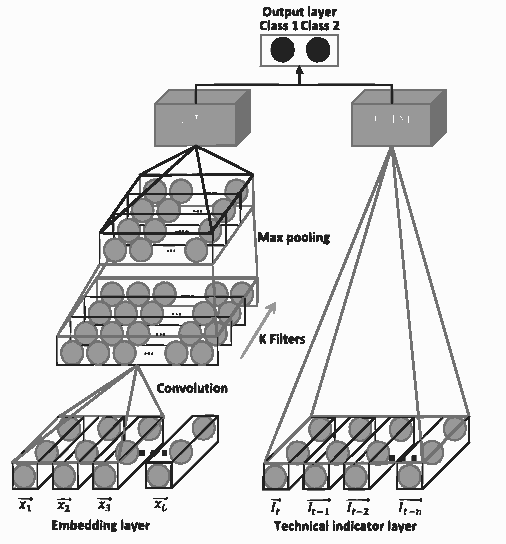
\includegraphics[width=0.6\textwidth]{./visuals/gr5.pdf}}
	\caption{Architecture of the RCNN model (from \cite{vargas2017deep}).}
\label{fig:gr5}
\end{figure}

According to the results discussed by the authors, the proposed RCNN model outperforms all other baseline models (NNs, RNNs and CNNs) with the exception of EB-CNN (event embedding CNN) which is also a powerful method for modeling content in news articles.

A more contemporary method for processing textual information and using it for forecasting time series is described in the publication \cite{lamon2017cryptocurrency}. The authors researched the ability of news and social media data to predict cryptocurrency prices. They used a modern pipeline consisting of:
\begin{itemize}
	\item a tokenizer to remove stop characters and punctuation (spaCy was used);
	\item a vectorizer to embed the tokenized text into numerical data;
	\item a classifier to learn feature weights (logistic regression and naive Bayes were chosen as the best performing algorithms for the task).
\end{itemize}
According to the published results, the models extracted general trends for price growth over the examined time period well, however predictions of daily price changes were quite inaccurate. Specifically, predicting fluctuations going against the general trend was a problem. Nonetheless, most of the predictions were correct, which implies the ability of non-technical data such as news to be used as predictors for financial variables.

As the next step in developing a working forecasting model powered by news headlines, the authors of the article \cite{li2022novel} have proposed a framework tuned for this task. The designed text-based framework (TBF) takes full advantage of the textual input data and predicts agricultural futures such as soybean prices. The structure of TBF is depicted in figure \ref{fig:gr6} (\cite{li2022novel}).
\begin{figure}[h!]\vspace*{4pt}
%\centerline{\includegraphics{fx1}\hspace*{5mm}\includegraphics{fx1}}
	\centerline{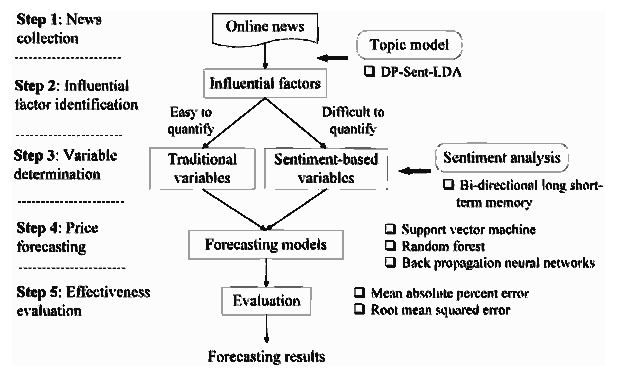
\includegraphics[width=0.8\textwidth]{./visuals/gr6.pdf}}
	\caption{Structure of the text-based framework (from \cite{li2022novel}).}
\label{fig:gr6}
\end{figure}

The framework combines tasks of topic analysis described in subsection \ref{ta}, sentiment analysis and time series forecasting. The most intriguing part of the framework is in the steps 2 and 3. The model identifies influential factors if those are easily quantifiable or performs sentiment analysis instead otherwise. This lets all the news to be utilized in model fitting without losing quality by including vague news.

For the forecasting section of the framework, the authors used SVR (support vector regression), RF (random forest) and BPNN (back propagation neural network). The authors compared all TBF-based models to baseline ARIMA. According to the results presented in the article, TBF-RF and TBF-SVR performed as well as ARIMA with small prediction horizon while TBF-BPNN had significantly higher forecasting errors. Interestingly, starting from lags of 40-50 days, prediction error of ARIMA starts growing linearly with the lag. TBF models' errors reach a plateau after 10-15 days and remain stable regardless how large is the time lag. Thus, in medium- and long-term predictions all of the TBF-based models outperform ARIMA.

Less task-specific methods were used by the author of the PhD thesis \cite{jeong2022predicting} in the task of Apple stock price forecasting. An array of conventional time series forecasting models allowing for exogenous context was used in conjunction with NLP methods for processing news headlines. For news sentiment analysis the following models were used:
\begin{itemize}
	\item LSTM (long short-term memory networks), a type of RNN discussed in subsection \ref{tsp}.
	\item GRU (gated recurrent unit) is a modified LSTM, where the addition of new information and retention of old information are interdependent.
	\item BERT (bidirectional encoder representation from transformers) is one of the cutting-edge NLP models with complicated architecture that takes advantage of transformers -- RNNs tuned for sequential information and NLP tasks.
\end{itemize}

For time series prediction the following methods were utilized:
\begin{itemize}
	\item (S)ARIMA(X), (seasonal) autoregressive integrated moving averages (with exogenous predictors) -- classical time series forecasting models discussed in subsection \ref{tsp}.
	\item Linear regression using PCA (principal component analysis), a method that performs dimension reduction and viewing the dependent variable as a linear combination of the predictors in the new latent space. 
	\item RF (random forest method) is an ensemble learning method that consists of multiple decision trees. Every tree produces its prediction and they all are averaged for the total forecast. 
	\item LSTM, described before.
\end{itemize}

According to the results presented in the article, SARIMAX failed to provide any accurate predictions in this task, while LSTM and, interestingly, linear regression with PCA had low MSE values of forecasts. Poor performance of SARIMAX could be explained by the lack of detail in the input data.

The forecasting methods that use text-based input for predicting financial time series were summarized in the table \ref{tab:t6}.

\begin{table}[h]
\centering
\caption{Comparison of time series forecasting methods.}
\label{tab:t6}
\resizebox{0.8\columnwidth}{!}{
\begin{tabular*}{\hsize}{@{\extracolsep{\fill}} p{2cm} p{2.5cm} p{4.5cm} p{4.5cm} l@{}}
\toprule
Method & Type & Benefits & Drawbacks & References \\
\colrule
ARX & autoregressive, parametric & simplicity, good performance for predictable time series & offers only a slight improvement over AR & \cite{mao2011predicting} \\
RCNN & RNN, \newline non-parametric & exceptional performance & complicated architecture, long optimization & \cite{vargas2017deep} \\
Tokenizer, vectorizer, logistic regression & parametric & good at trend extraction & problems with anomalies & \cite{lamon2017cryptocurrency} \\
TBF & non-parametric & exceptional performance, effective usage of all input news & complicated architecture makes the model hard to modify for other tasks & \cite{li2022novel} \\
SARIMAX & autoregressive, parametric & good performance, seasonality modeling, simplicity & outperformed by NNs & \cite{jeong2022predicting} \\
LR with PCA & parametric & simplicity, small number of parameters & usually deals only with predictable data & \cite{jeong2022predicting} \\
RF & non-parametric & good performance, ensemble strategy & usually outperformed by NNs & \cite{jeong2022predicting} \\
LSTM & RNN, \newline non-parametric & excellent performance, ability to model complicated patterns & performance highly dependent on the quality of input data & \cite{jeong2022predicting} \\
\botrule
\end{tabular*}
}
\end{table}

\newpage

\subsection{Choice of methodologies} \label{com}

Based on the overview of related scientific work, BERTopic was chosen as the method for processing textual news information for its exceptional performance and stability across several languages and ARIMAX was chosen for forecasting consumer time series for its simplicity and efficiency.

As transactional datasets are often confidential and publication of the raw data is restricted, synthetic datasets offer identical consumption distributions without showing any of the initial clients. For synthesizing categorized time series of financial transactions, an autoencoder capable of extending real datasets with synthetic time series was proposed. It was developed in such a way that the statistical parameters of the resulting dataset are identical to those of the initial one. The autoencoder consists of three dense hidden layers of sizes 64, 32 and 64, accordingly. The model takes a 2D-array of real world temporal data and outputs it as another 2D-array but with the number of time series chosen by the user. The structure of the model is described in figure \ref{fig:gr7}.
\begin{figure}[h!]\vspace*{4pt}
%\centerline{\includegraphics{fx1}\hspace*{5mm}\includegraphics{fx1}}
	\centerline{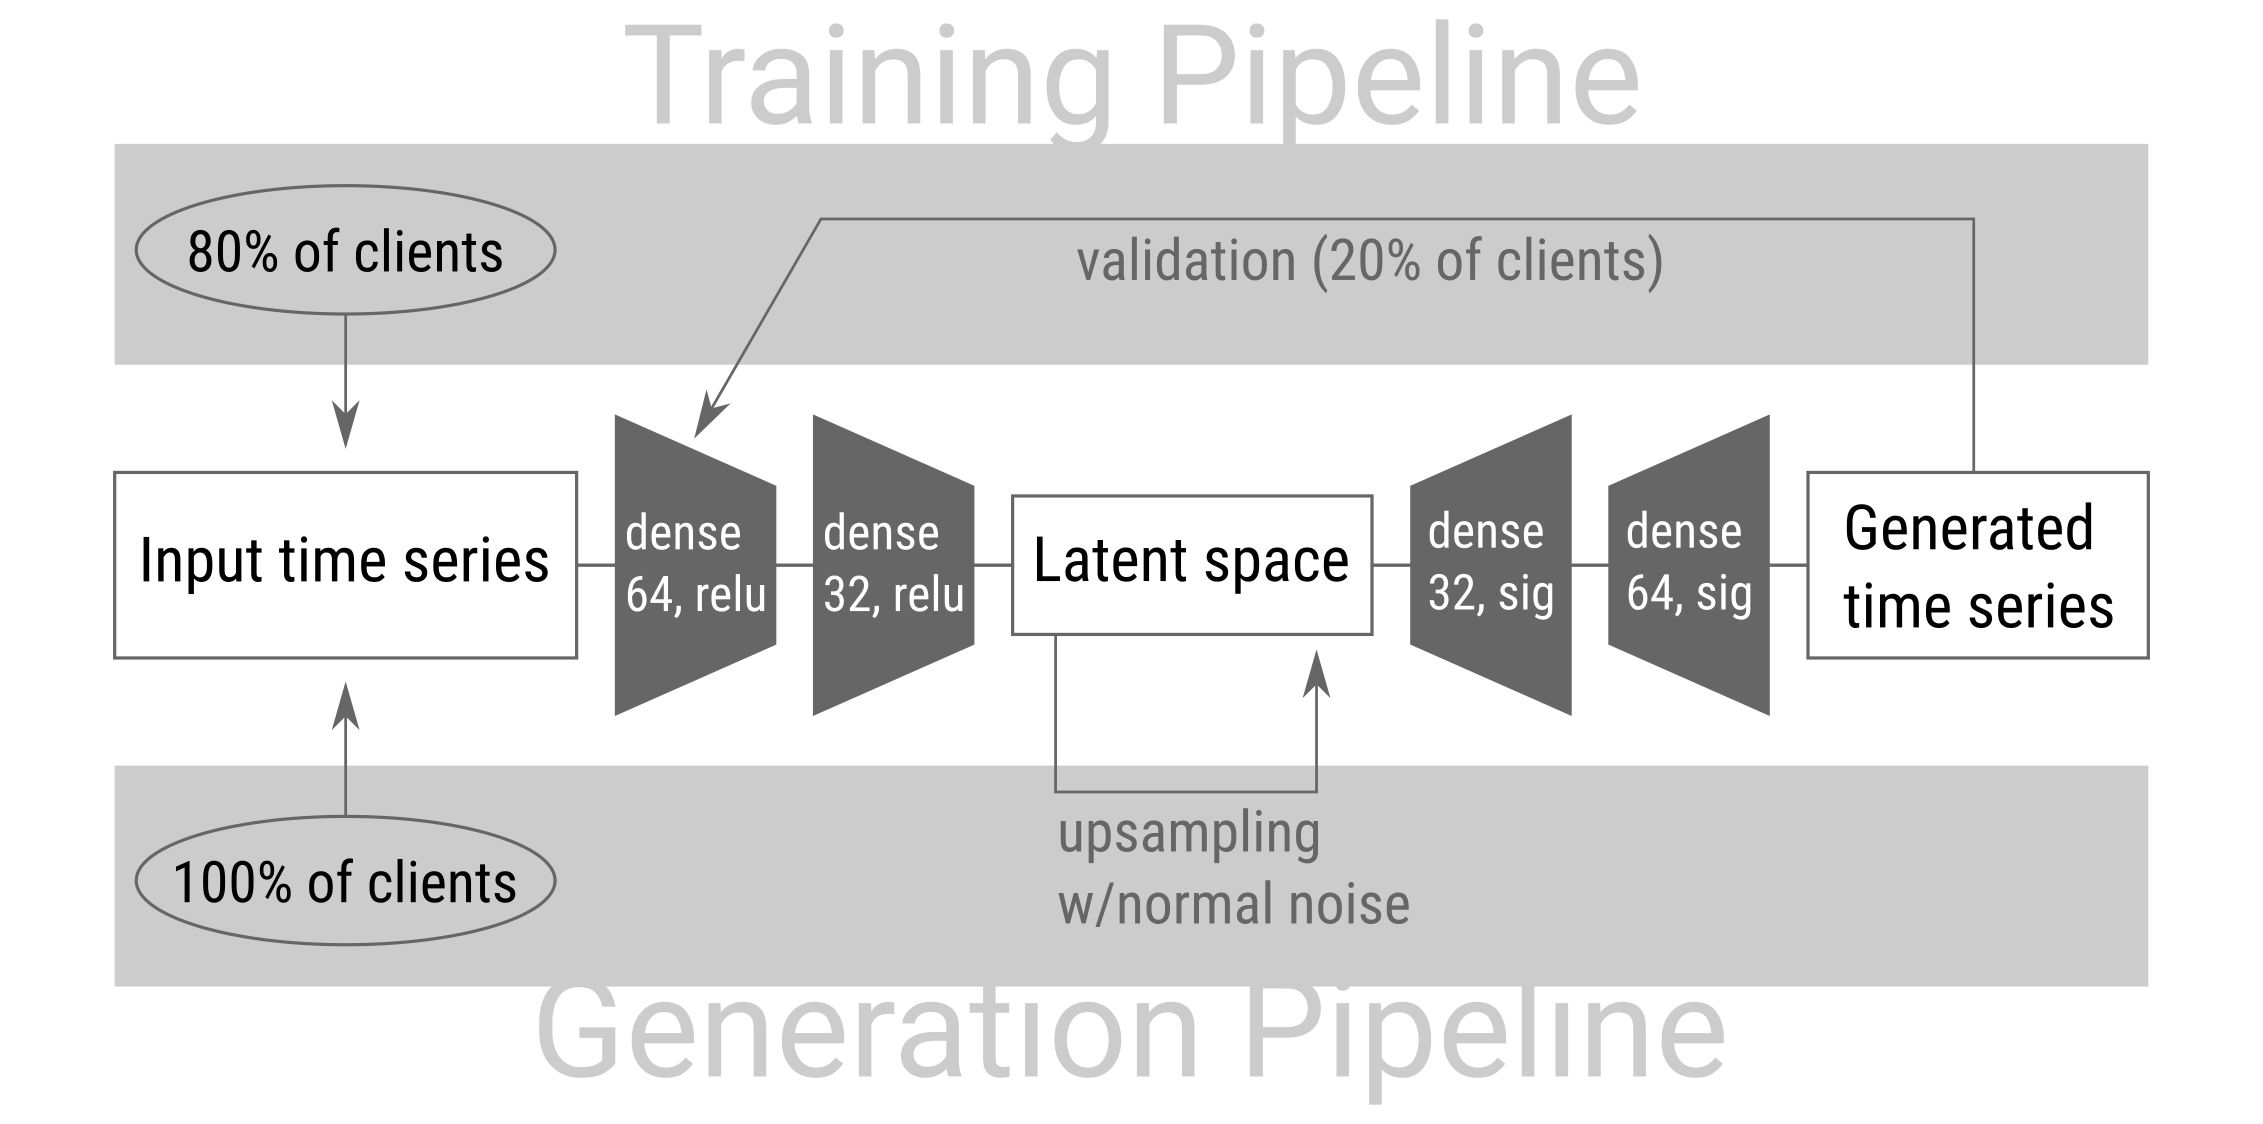
\includegraphics[width=0.8\textwidth]{./visuals/gr7.png}}
\caption{Structure of the autoencoder for transactional dataset synthesis.}
\label{fig:gr7}
\end{figure}

Every time series vector in the output data is a modification of one of the vectors from the initial set. The modification is applied in the latent space, where the vectors have a lower dimension, in form of noise. This approach guarantees similarity of the two datasets and lowers the runtime of the algorithm in comparison to modifying the time series vectors as-is.

This model was tested on 14 datasets of consumption data. Pearson's cross-correlation between the initial and the resulting time series was maximal with a time lag of 0 and its values ranged from $0.985$ to $0.998$. Thus, the two datasets are effectively identical and the autoencoder is applicable for the task of dataset extension.

For the task of topic analysis, BERTopic, text clusterization tool leveraging BERT embedders, was used. The structure of BERTopic was described in the literature overview and in the corresponding article \cite{grootendorst2022bertopic}. In a nutshell, it is composed of:
\begin{enumerate}
	\item BERT-embedders based on transformers -- models tuned for extracting semantic relationships. For russian language, embedding is done via ``distiluse-base-multilingual-cased-v1" pretrained models.
	\item UMAP dimension reduction.
	\item HDBSCAN clustering: every sentence within a cluster is concatenated and the words in the resulting sentence are gathered in a pool with word frequencies called bag-of-words. Every cluster is characterized by one. For topic representation, c-TF-IDF is used (a metric for the importance of a certain word within a cluster). The algorithm chooses word characteristic for the cluster and forms a topic from them.
\end{enumerate}
In this scientific work lemmatization of sentences before topic analysis is performed with help of NLTK multilingual dictionaries.

For time series forecasting, autoregressive ARIMAX models were used as they are easy to implement, efficient and they allow for the usage of exogenous variables. As the model is parametric, it has three parameters: $p$ -- the AR order (number of time lags), $d$ -- the integration parameter (number of times differencing is performed to make the time series stationary) and $q$ -- the order of the MA model (number of time lags). ARIMAX $(7,1,7)$ was used in this work. Parameters $p$ and $q$ were chosen to be $7$ so as to capture any remnant weekly patterns after the deletion of seasonality. Parameter $d$ was chosen to be $1$ to make all the time series used in this work stationary. This was proven by ADF-tests.

\newpage

\subsection{Data and experiments}
\vspace{-3mm}
\subsubsection{Data mining, synthesis and processing}

14 sets of transactional temporal data were processed by the autoencoder described in section \ref{com}. Every dataset contains financial transactions from 2020/01/01 to 30/09/2020 in one of the 14 consumption categories.

News information used in the main part of this research was acquired via scripts scraping five news websites listed in figure \ref{fig:gr8}.
\begin{figure}[h!]\vspace*{4pt}
%\centerline{\includegraphics{fx1}\hspace*{5mm}\includegraphics{fx1}}
	\centerline{
\includegraphics[width=0.7\textwidth]{./visuals/gr8.png}}
\caption{The sources of news headlines.}
\label{fig:gr8}
\end{figure}

Headlines of news articles with the corresponding dates of publication were chosen as the contextual dataset. In total, about 78000 headlines were scraped.

The raw news headlines were lemmatized via NLTK dictionaries. Dynamical topic modeling was performed using BERTopic with the window size of 7 days. The model's output was a set of weekly time series for the popularity of topics in the news. These time series were then interpolated by quadratic spline to acquire daily series. Further processing included manual deletion of irrelevant topics and summation of semantically similar topics. Finally, a set of 13 topic popularity time series was obtained.

In this research work the news contextual time series were extended by other open-source context information such as macroeconomical parameters and COVID-19 statistical data. 20 time series from 8 sources listed in figure \ref{fig:gr9} were interpolated with quadratic spline to obtain daily series.

The sources depicted in figure \ref{fig:gr9} contained the following data:
\begin{enumerate}
\item Mortgage rates in Russia;
\item USD exchange rate;
\item Unemployment;
\item Key interest rate and inflation;
\item GDP;
\item Real estate affordability;
\item Consumer price index;
\item COVID-19.
\end{enumerate}

\begin{figure}[h!]\vspace*{4pt}
%\centerline{\includegraphics{fx1}\hspace*{5mm}\includegraphics{fx1}}
	\centerline{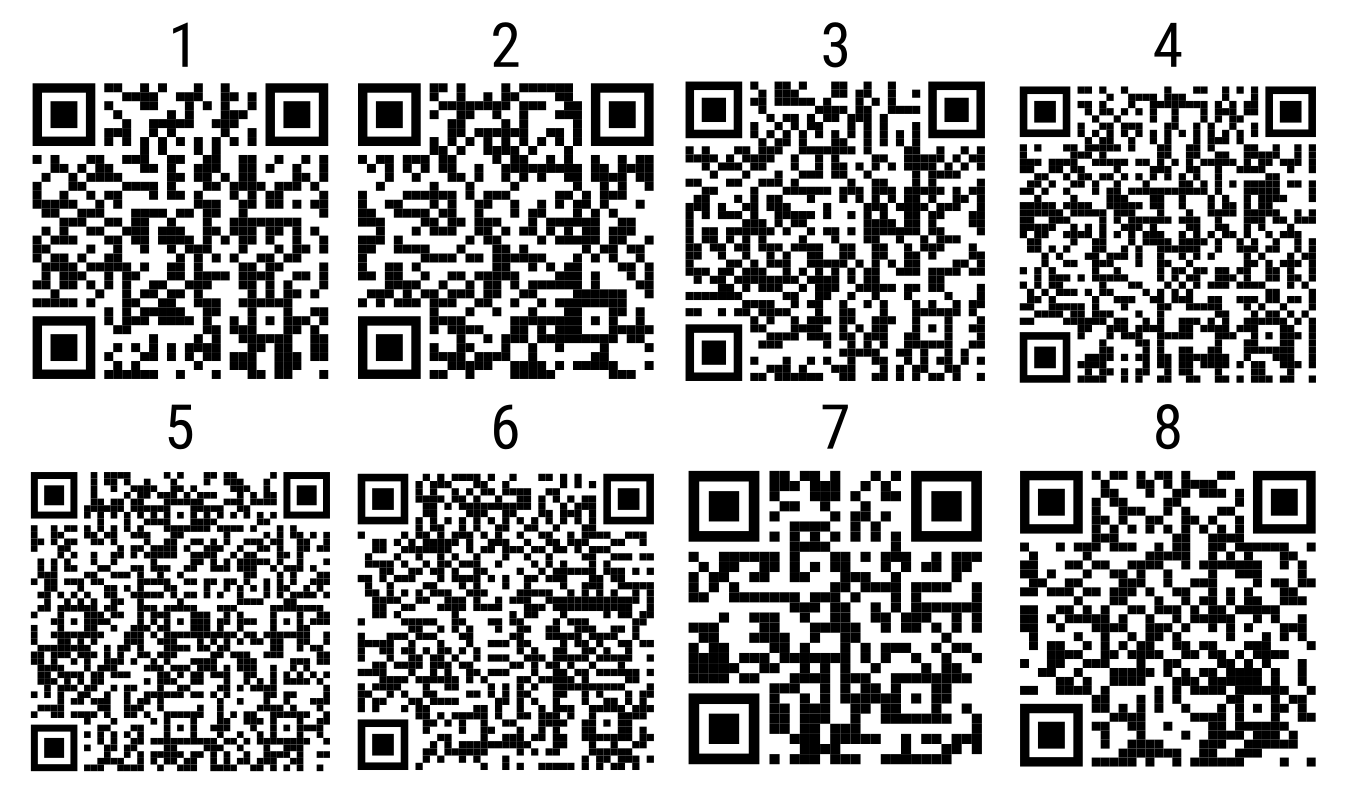
\includegraphics[width=0.6\textwidth]{./visuals/gr9.png}}
\caption{The sources of other context information.}
\label{fig:gr9}
\end{figure}

\subsubsection{The impact of context information on consumer behavior}

It was hypothesized that consumer behavior forecasting can serve as a method for studying the influence of context on consumption. In fact, to study the patterns in stochastic processes, either the analysis of the statistical characteristics of the time series or models capable of predicting them are utilized. The latter approach is more illustrative, and at the same time more applied to real world tasks, as the assessment of future changes in processes is useful in any business. Thus, analyzing the impact of context composition on the quality of predictive models is effectively equivalent to examining the impact of context on consumer activity itself. 

ARIMAX autoregressive models were used as a time series prediction tool. It should be noted that:
\begin{itemize}
	\item Individual client series were summed to form a dataset of 14 series where each one represents daily spendings of the whole population of clients on one of the 14 categories.
	\item Time series trends without the seasonal term were used for fitting the models. Seasonal decomposition was performed using the statsmodels library of the Python3 language.
\end{itemize}
Then, as additional preprocessing measures, the time range of the datasets was narrowed from 2020/01/01-2020/09/30 to 2020/04/01-2020/09/30. This is due to the non-stationarity of the time series during the first three months of 2020.

The results of this and subsequent experiments were ensured to be representative by carrying out each prediction 10 times, with different partitioning of the data into training and test subsets. In this paper, the starting date of the training dataset is 2020/04/01, and the starting dates of the test series range from 2020/09/10 up to 2020/09/20. The end date of the test series is 2020/09/30. The error metrics were averaged over these 10 attempts. 

The \textit{first experiment} consisted of predicting consumer activity using all available context simultaneously. The results of the ARIMAX prediction fit on all contextual information were unsatisfactory (rRMSE, relative RMSE of 51\% for category ``food"). 

Therefore, it was necessary to select certain exogenous variables and categories of consumption. This was done by fitting models on the variables individually to determine their viability as context. Those individual rRMSE values were plotted against exogenous variables and the consumption category in figures \ref{fig:gr10} and \ref{fig:gr11}. Only a selection of the variables and categories is presented for legibility.

\begin{figure}[h!]\vspace*{4pt}
\centerline{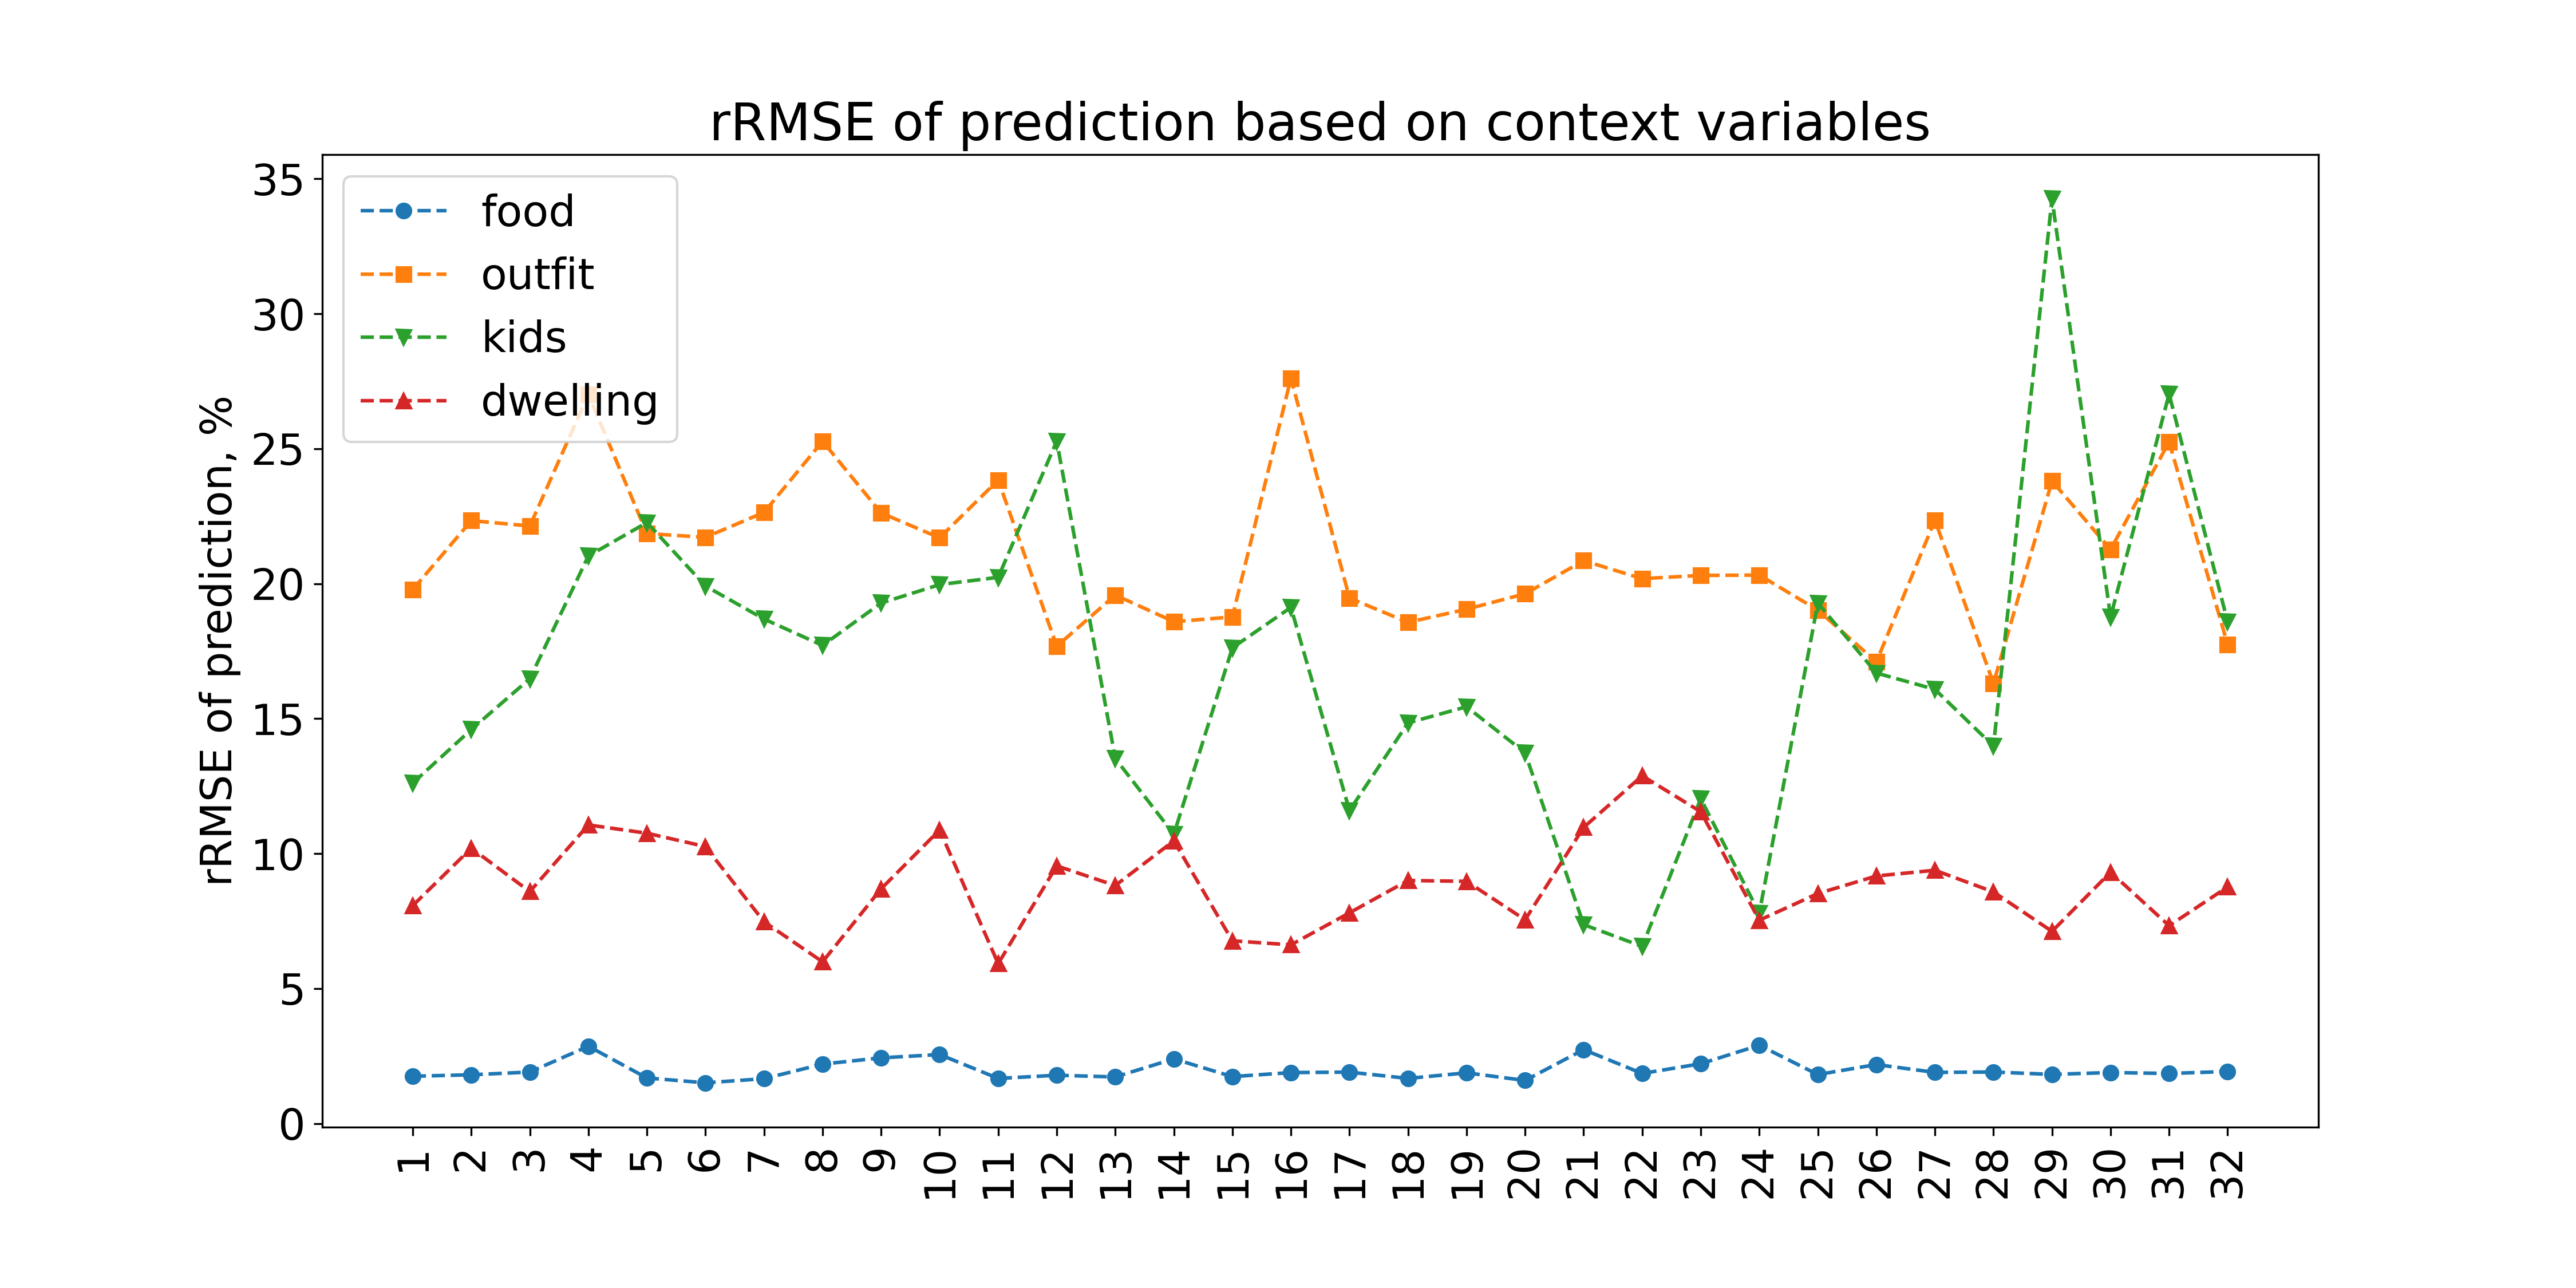
\includegraphics[width=0.8\textwidth]{./visuals/gr10.png}}
\caption{rRMSE of prediction for different exogenous variables.}
\label{fig:gr10}
\end{figure}

\begin{figure}[h!]\vspace*{4pt}
\centerline{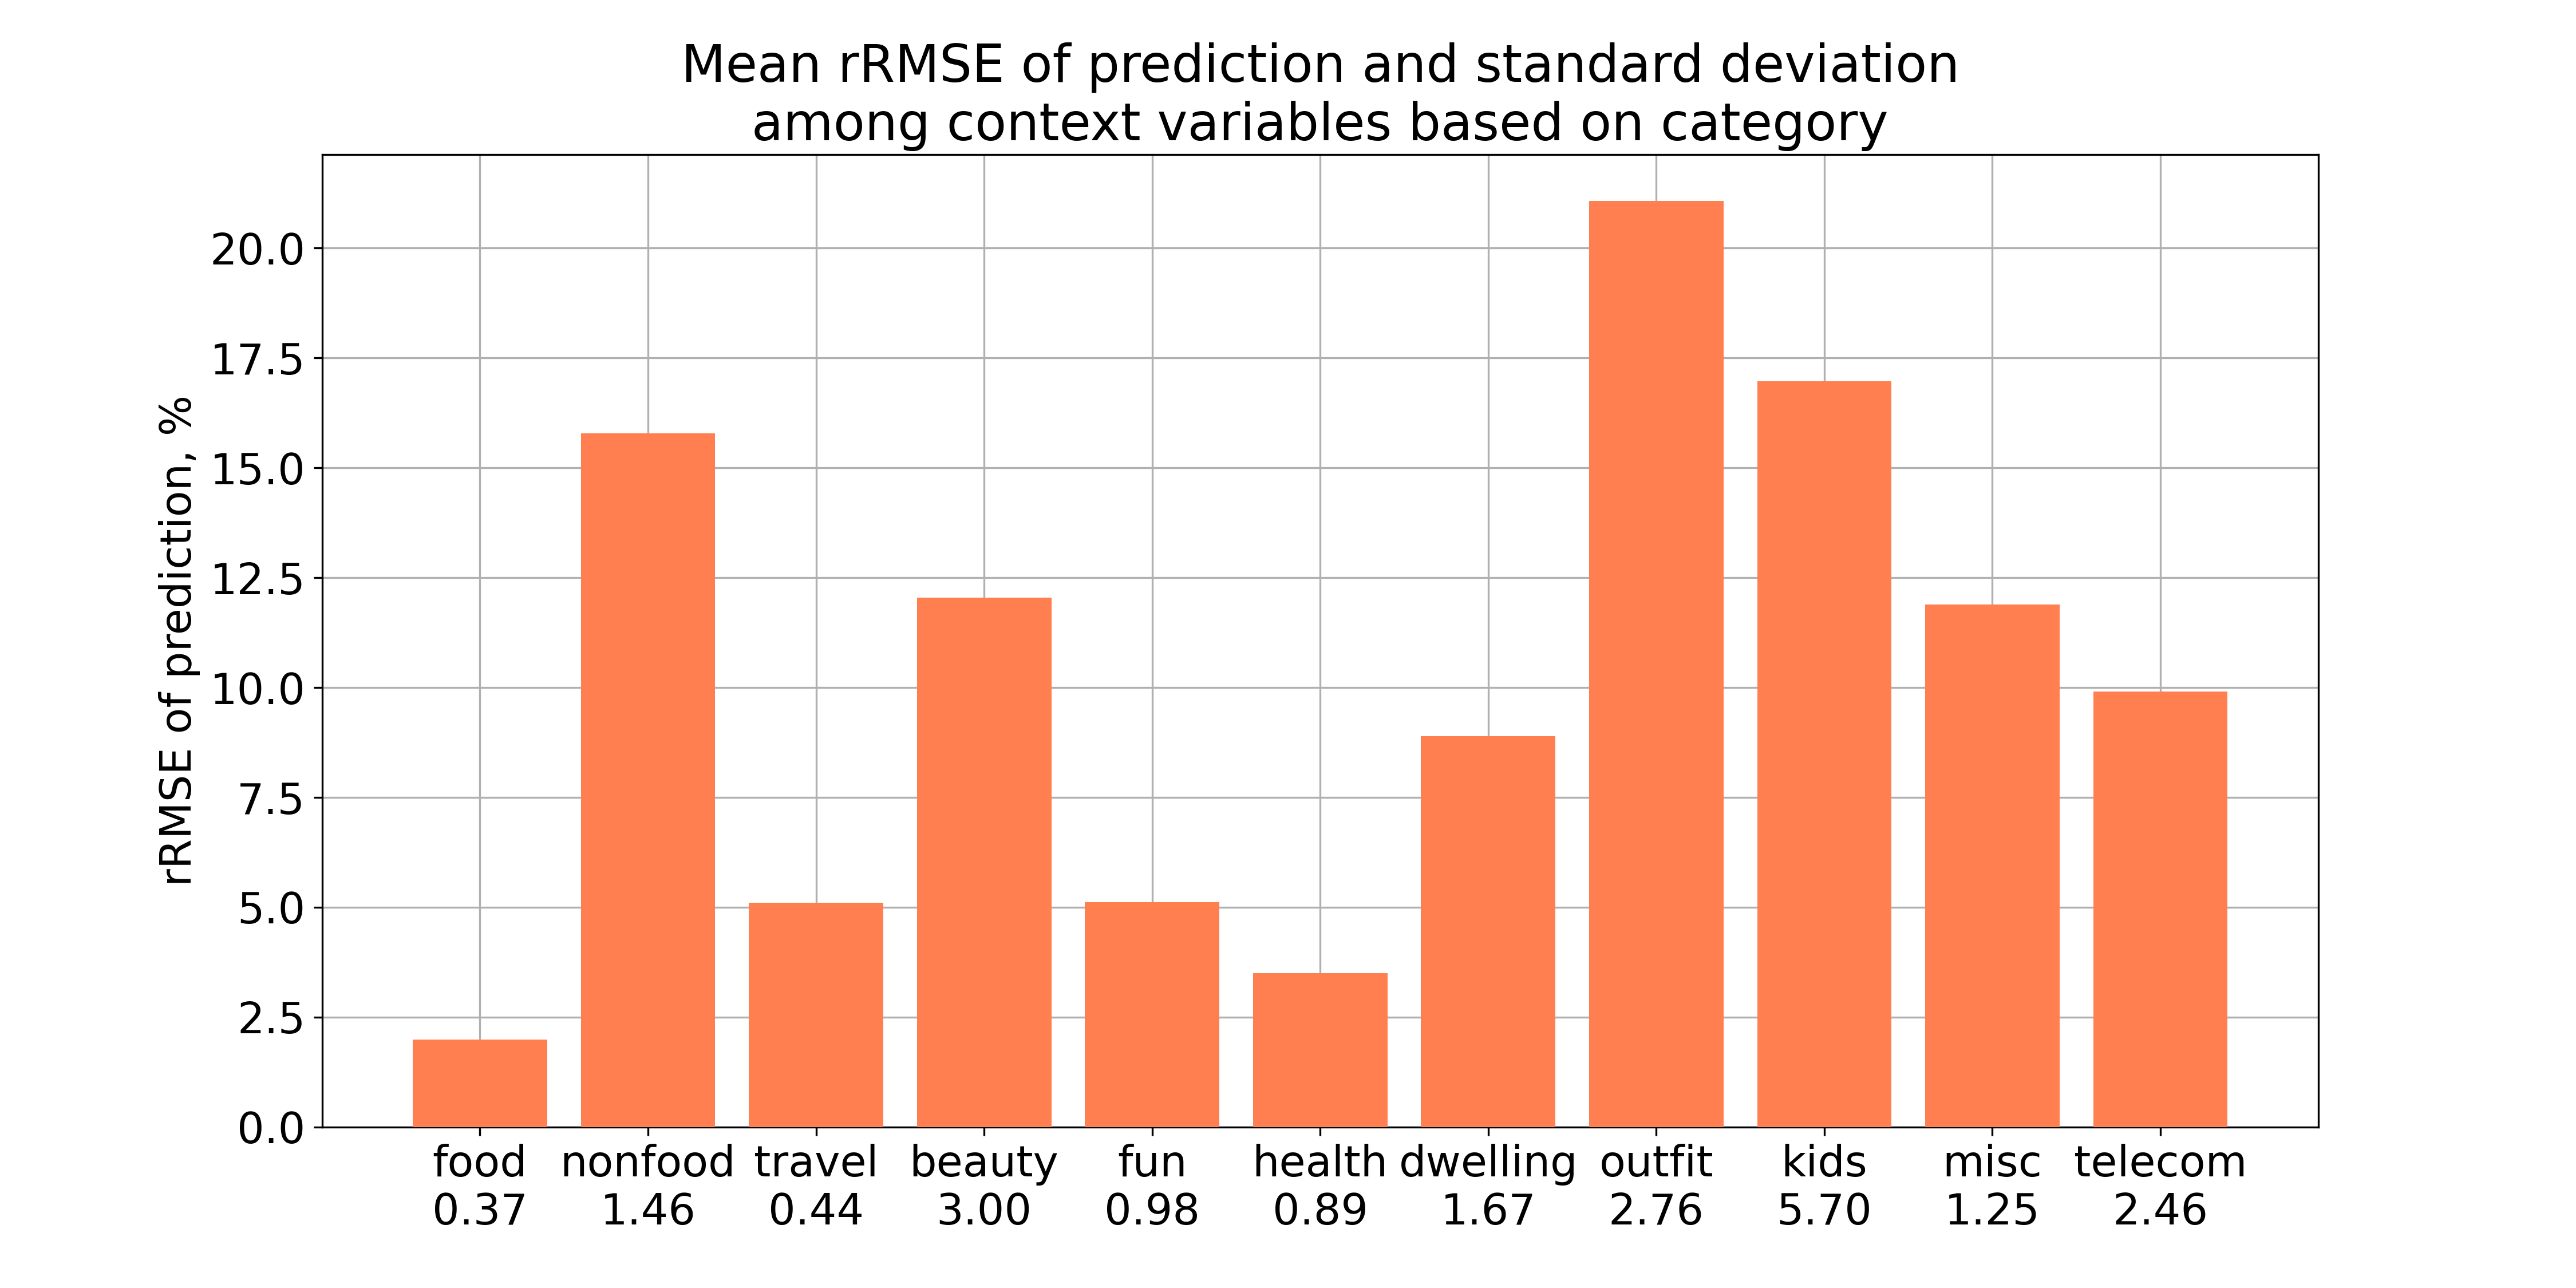
\includegraphics[width=0.8\textwidth]{./visuals/gr11.png}}
\caption{Mean rRMSE of prediction and its standard deviation across exogenous variables for consumption categories.}
\label{fig:gr11}
\end{figure}

Figure \ref{fig:gr10} shows that there are no exogenous variables which yield low-quality predictions across all categories. Thus, all have to be included in the research. Figure \ref{fig:gr11} gives motivation for two experiments. Firstly, the most accurate models are built for the categories ``food", ``travel", ``entertainment" and ``health". Secondly, the greatest variation in the quality of predictions for different contextual themes is observed in the categories ``beauty" and ``children". 

The \textit{second experiment} consisted of fitting ARIMAX models on the most predictable topics (``food", ``travel", ``entertainment" and ``health"). The five exogenous variables with the lowest individual prediction rRMSE values were used to build the models. Predictions for the mentioned consumption categories were of exceptional quality with forecasting errors ranging from 1.6\% to 4.46\%. An example forecast for the category ``food" is illustrated in figure \ref{fig:gr12}. Consequently, selecting the most appropriate exogenous variables can significantly improve prediction quality compared to using the entire context at once.
\begin{figure}[h!]\vspace*{4pt}
\centerline{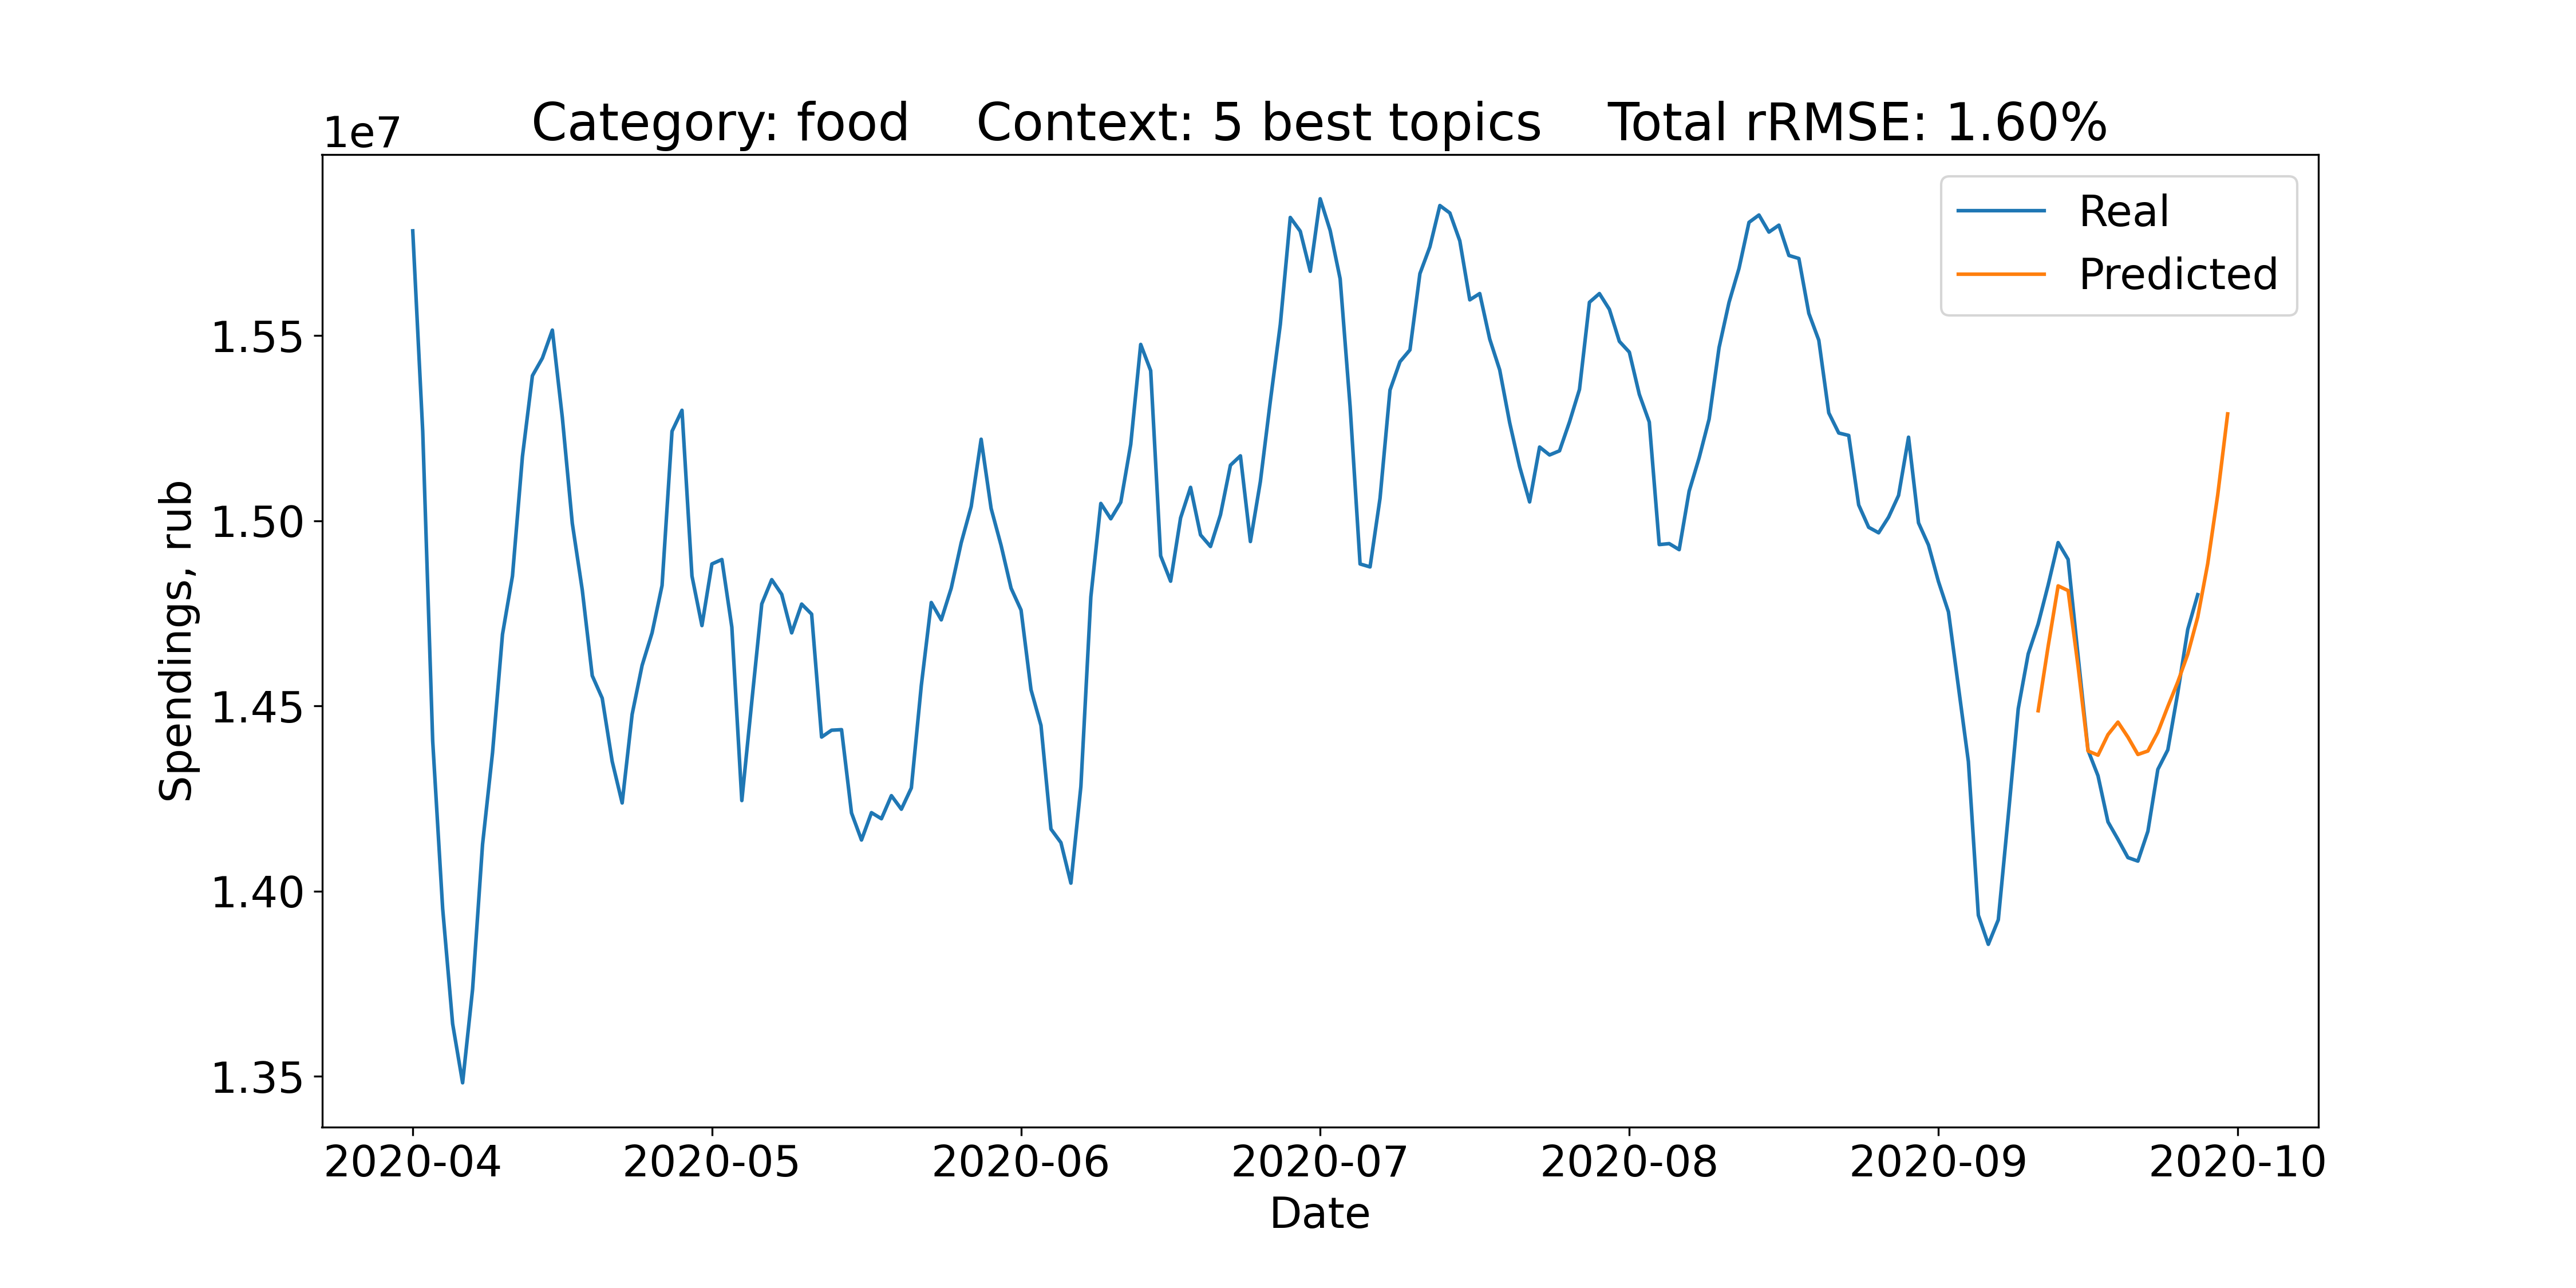
\includegraphics[width=0.8\textwidth]{./visuals/gr12.png}}
\caption{Forecasts for category ``food".}
\label{fig:gr12}
\end{figure}

The \textit{third experiment} is opposed to the previous one: if it is possible to improve the quality of the model by moving from all contextual variables to a subset of best performing ones, is it possible to improve the quality of the prediction by adding new exogenous variables to the context? The categories ``beauty" and ``children", the categories with the greatest variation in model quality across contextual variables, were chosen to illustrate this hypoithesis.

For the categories ``beauty" and ``children" ARIMAX models were constructed for all exogenous variables with individual rRMSE values in the ranges of 7.5-15\% and 10-23\%, respectively. The predictors with the lowest individual rRMSE (``Consumer Price Index", ``Consumer Price Index, Food" for ``beauty" and ``Consumer Price Index", ``Consumer Price Index, Food" and ``Consumer Price Index, Services" for ``children") were then added to the context. The addition of new exogenous variables reduced the rRMSE of the predictions by a factor of 3-4 times (from 20-30\% to about 7\%). An example forecast for ``children" is presented in figure \ref{fig:gr13}. It is worth noting that all added exogenous variables are negatively correlated with consumer activity with the lag of 0 days.
\begin{figure}[h!]\vspace*{4pt}
\centerline{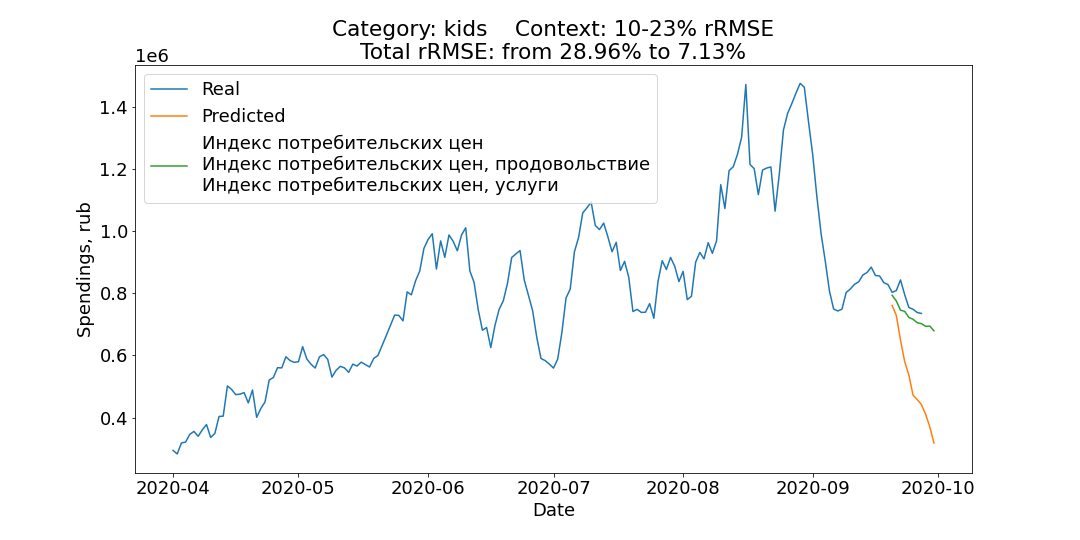
\includegraphics[width=0.8\textwidth]{./visuals/gr13.png}}
\caption{Forecasts for category ``children" before and after the addition of new variables.}
\label{fig:gr13}
\end{figure}

Thus, the addition of exogenous variables to the ARIMAX model also can significantly improve the quality of its prediction. 

In addition to predicting transactional time series, the maximum absolute values of the Pearson cross-correlation and the corresponding time lags in days were calculated. The values of the shifts and cross-correlation are shown in table \ref{tab:t7}. The cells corresponding to the best topics on which the models were built are highlighted in bold.

The most interesting cases are those where the absolute values of Pearson cross-correlation are high and the corresponding time lags have low values. For example, spendings on category ``travel" (which include public transport) and news about COVID-19 are negatively correlated with a lag of 3 weeks, which means that people are less likely to use means of public transport soon after they hear news about the pandemic.

\begin{table}[!h]
\centering
\caption{Pearson cross-correlation between consumption and exogenous predictors.}
\label{tab:t7}
\resizebox{0.8\columnwidth}{!}{
	\begin{tabular*}{\hsize}{@{\extracolsep{\fill}} p{4.6cm} llllll@{}}
\toprule
 & \textbf{food} & \textbf{travel} & \textbf{beauty} & \textbf{fun} & \textbf{health} & \textbf{kids} \\
\colrule
\textbf{Unemployment} & 113, -0.81 & \textbf{22, 0.94} & 42, 0.95 & 26, 0.86 & 1, 0.83 & 0, 0.74 \\
\textbf{Covid-19 in Russia, total deaths} & 95, -0.80 & 0, 0.89 & 0, 0.95 & \textbf{0, 0.87} & 0, 0.73 & 0, 0.69 \\
\textbf{Key interest rate} & 103, 0.82 & \textbf{18, -0.95} & 36, -0.95 & 26, -0.88 & 0, -0.83 & 0, -0.73 \\
\textbf{COVID news} & 97, 0.81 & \textbf{21, -0.93} & 22, -0.91 & 18, -0.85 & \textbf{0, -0.81} & 0, -0.74 \\
\textbf{Travel news} & 94, -0.76 & 122, -0.66 & 84, 0.56 & \textbf{35, 0.54} & 35, 0.51 & 71, 0.65 \\
\textbf{Investment news} & \textbf{39, 0.61} & 117, 0.45 & 72, 0.61 & 116, 0.59 & 117, 0.65 & 93, -0.42 \\
\textbf{GDP, billions rub} & 83, -0.81 & 0, 0.82 & 0, 0.91 & \textbf{0, 0.83} & \textbf{0, 0.69} & 0, 0.66 \\
\textbf{Mortgage rates, sec. market} & \textbf{113, 0.80} & 0, -0.89 & 0, -0.94 & 0, -0.85 & 0, -0.73 & 0, -0.75 \\
\textbf{USD exchange rate, rub} & 96, 0.80 & \textbf{49, -0.77} & 58, -0.86 & 37, -0.62 & 31, -0.62 & 68, -0.67 \\
\textbf{Real estate affordability, SPb} & 122, -0.72 & 0, 0.88 & 19, 0.91 & 0, 0.79 & \textbf{0, 0.68} & 16, 0.77 \\
\textbf{Consumer price index, services} & 75, -0.74 & 104, 0.53 & 122, 0.68 & 104, 0.38 & 121, 0.17 & \textbf{115, 0.83} \\
\textbf{Annual inflation, \%} & 91, -0.76 & 0, 0.87 & 8, 0.93 & \textbf{0, 0.85} & 0, 0.71 & 113, -0.80 \\
\textbf{Mortgage rates} & \textbf{111, 0.81} & 22, -0.90 & 45, -0.91 & 30, -0.85 & 1, -0.78 & 0, -0.78 \\
\textbf{Consumer price index} & 122, 0.72 & 63, -0.75 & \textbf{86, -0.80} & 56, -0.68 & 55, -0.57 & \textbf{0, -0.75} \\
\textbf{Consumer price index, food} & 122, 0.68 & 8, -0.81 & \textbf{24, -0.84} & 13, -0.74 & 13, -0.65 & \textbf{13, -0.74} \\
\botrule
\end{tabular*}
}
\end{table}

\clearpage

\section{Findings} \label{f}

As part of this research, methods for mining and processing news headlines and other contextual information were developed and implemented in Python3. In addition, a method for synthesizing transactional data based on real-world data was proposed. 

Consumer activity of was modeled using ARIMAX autoregressive models. The best prediction quality is achieved by careful selection of the context variables on which the model is fit. The predictive ability of the model, depending on the consumption category, can be improved both by reducing the number of exogenous variables and by adding new ones. As a result, highly accurate forecasts can be acquired, as illustrated in figure \ref{fig:gr14}.
\begin{figure}[h!]\vspace*{4pt}
	\centerline{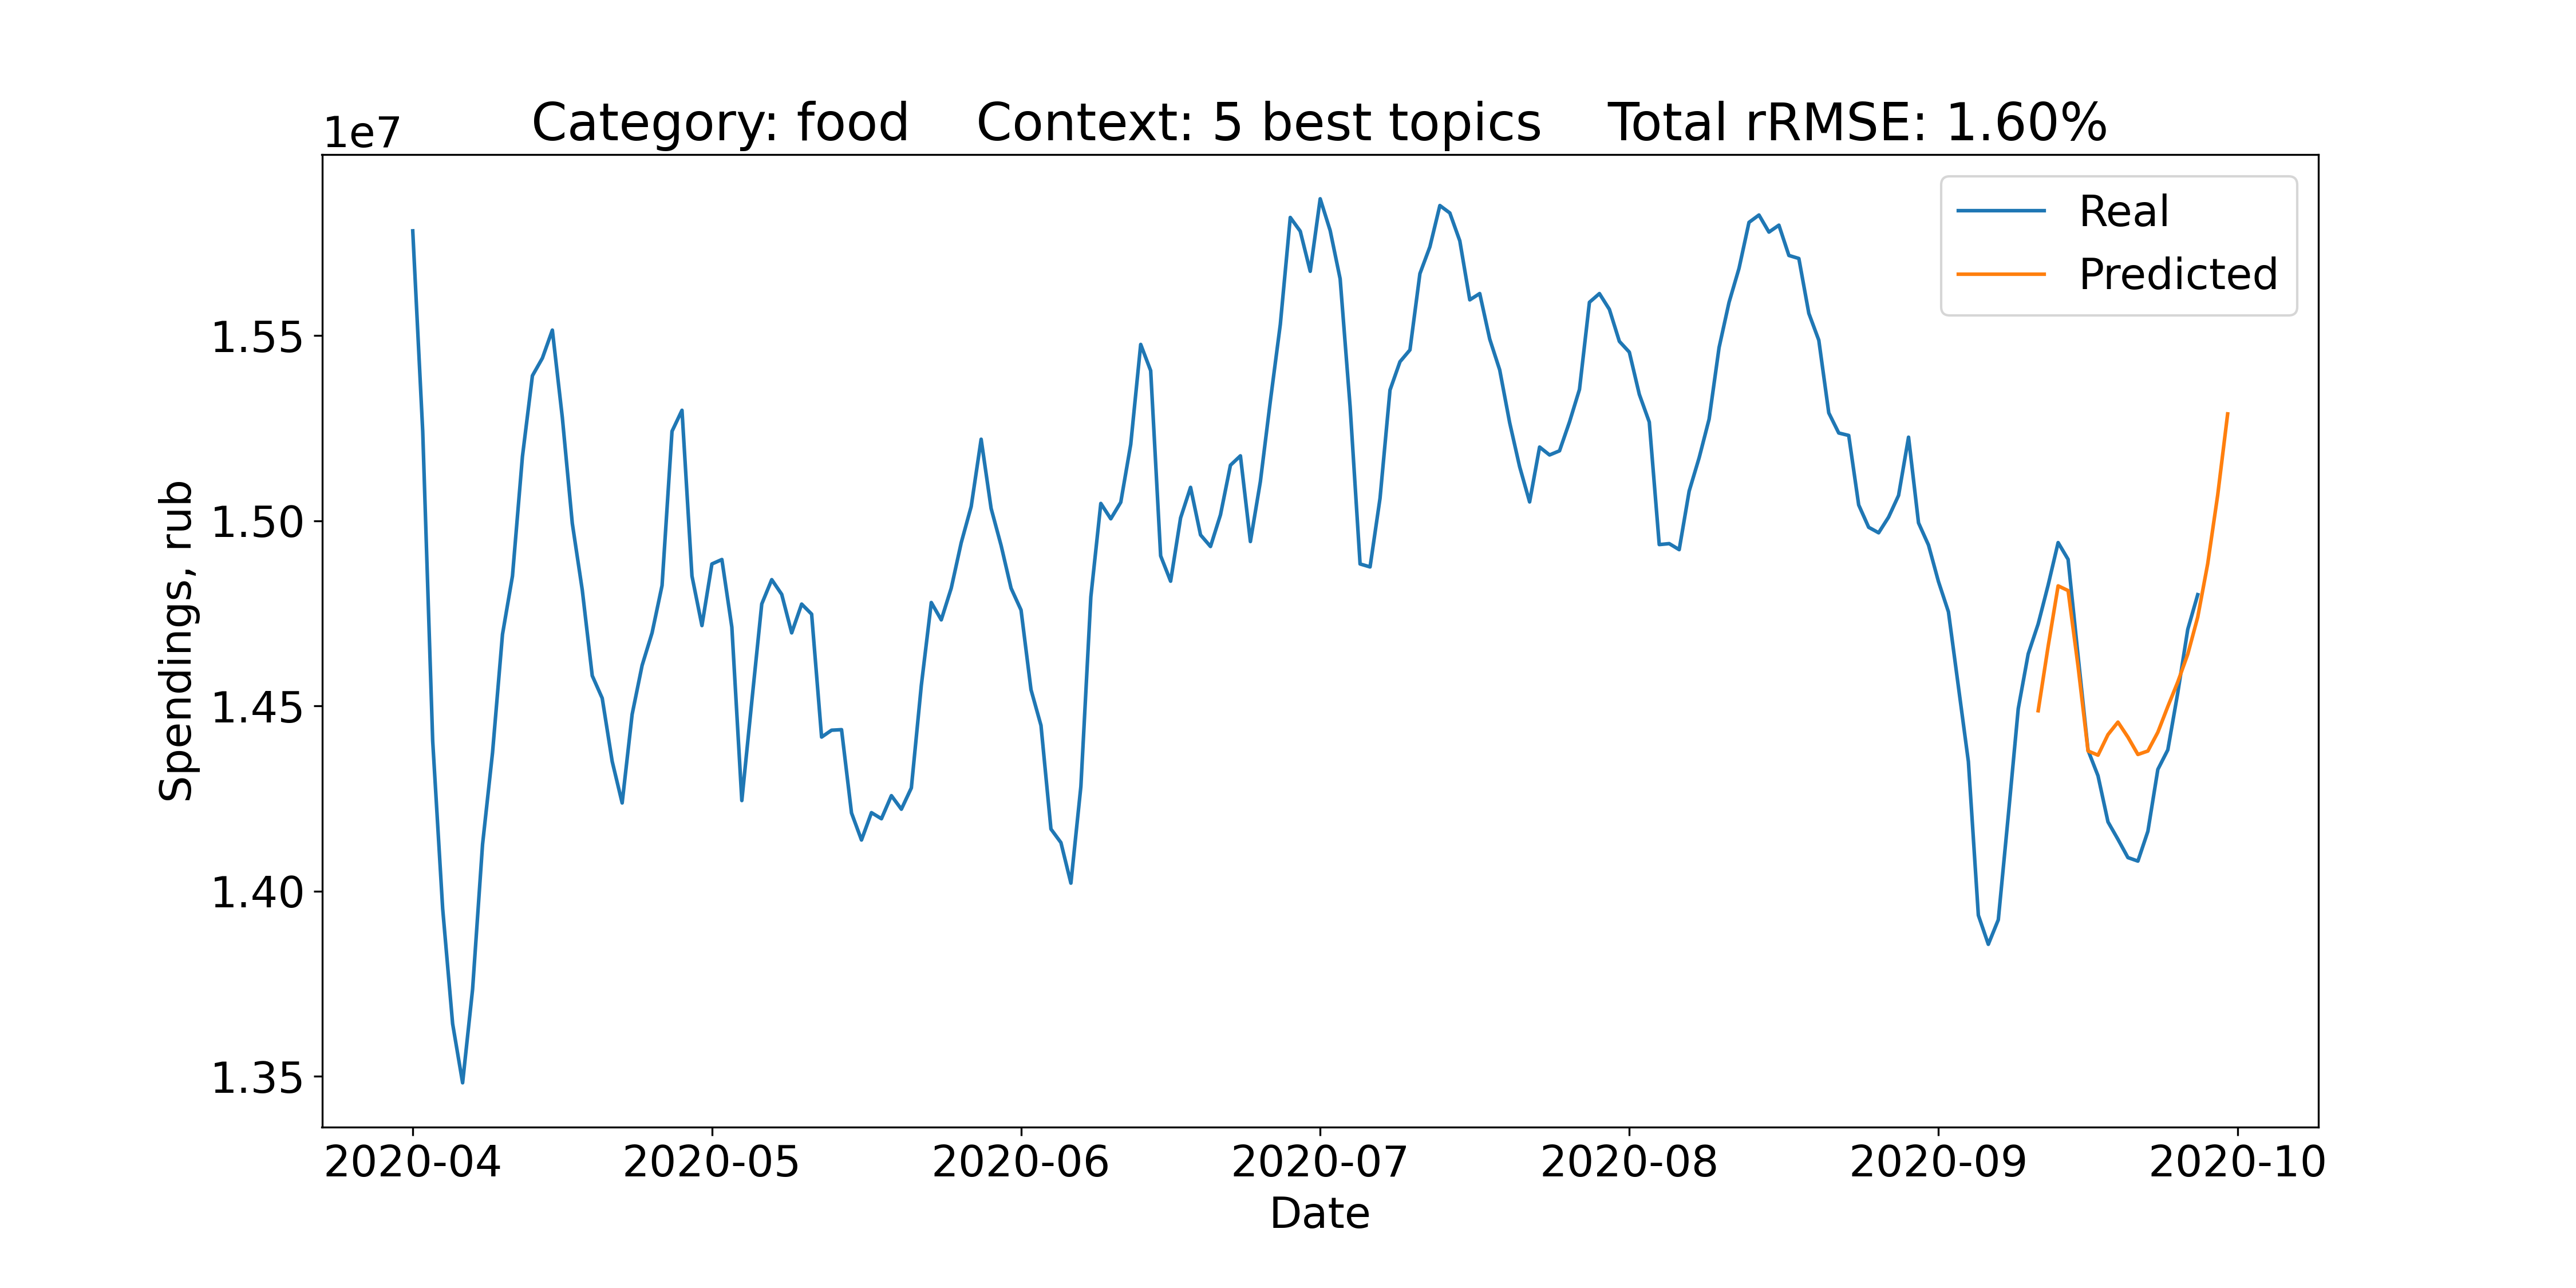
\includegraphics[width=0.49\textwidth]{./visuals/gr12.png}\hspace{1mm}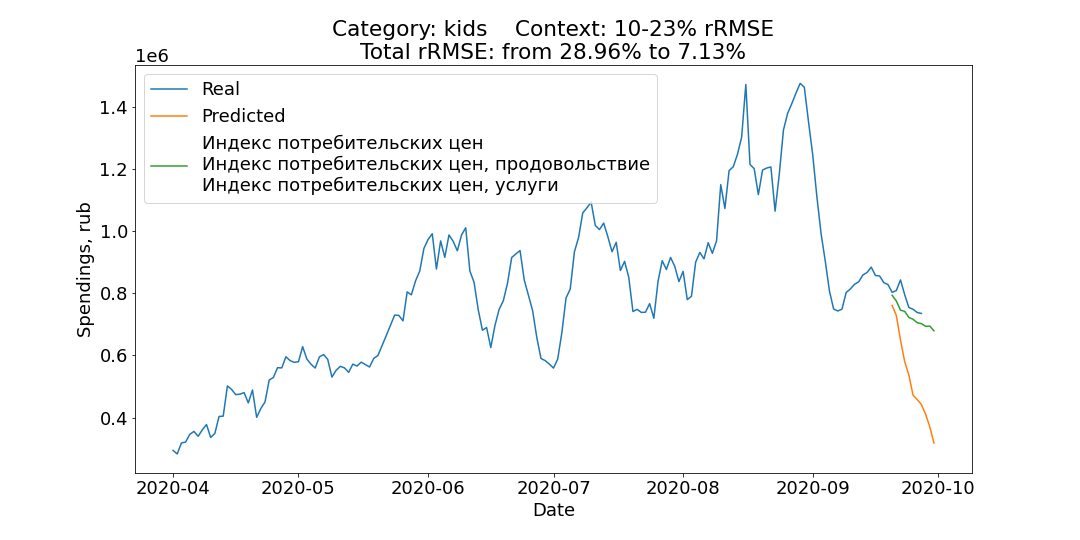
\includegraphics[width=0.49\textwidth]{./visuals/gr13.png}}
\caption{Consumption forecasts with limited context (left) and extended context (right).}
\label{fig:gr14}
\end{figure}

Thus, it is shown that the use of contextual information can improve the prediction accuracy of transactional time series. Consequently, there is some causal relationship between contextual information and modeled consumer behavior. However, not all categories of consumption were able to yield high prediction accuracy, leading to the conclusion that consumption in some categories is not causally related to the contextual information considered.

In addition, the cross-correlation of context and consumer time series with a time shift can be used to confirm or refuse hypotheses about the causal relationship between context and consumption. For example, a strong correlation with relatively small shifts can provide clues about the consumer's direct response to the changing context. 

\section{Conclusion}

During the internship, the Individual task was fully completed, which is depicted in the section \ref{f}. Planned practice results were fully achieved, however, more detailed endeavor into the topic of research is needed for more fundamental understanding of the problem, which will be the next step regarding this work.

\newpage

%\section*{Acknowledgements}
%\addcontentsline{toc}{section}{Acknowledgements}

%I would like to express my sincere gratitude to my supervisor Anton Kovantsev who supported the choice of the topic and made this research possible. His assistance throughout the process of conducting this research helped it become more logically structured and helpful for the audience. I would also like to give special thanks to my family and close friends for their continuous support and understanding.

\bibliography{./nir-bib.bib}{}
\addcontentsline{toc}{section}{References}
\bibliographystyle{unsrt}

\end{document}
